\documentclass[10pt,preprint2]{aastex}
\usepackage[a4paper,asymmetric,left=0.75in,right=0.75in,top=0.75in,bottom=0.75in]{geometry}
\AtBeginDocument{\newgeometry{asymmetric,left=0.75in,right=0.75in,top=0.75in,bottom=0.75in}\hoffset=0pt\setlength{\columnsep}{0.3in}\pagestyle{fancy}\fancyhf{}\fancyhead[L]{\small ASTRON 128 Astronomy Data Science Laboratory}\fancyhead[R]{\small Lab 1}\fancyfoot[C]{\thepage}}
\usepackage{amsmath, amsfonts, amssymb}
\usepackage{hyperref}
\usepackage{graphicx}
\usepackage{tikz}
\usepackage{booktabs}
\usepackage{fancyhdr}
\setlength{\headheight}{11pt}
\addtolength{\topmargin}{-0.16pt}
\usepackage{float}
\usepackage{stfloats}
\usepackage{pdflscape}
\usetikzlibrary{arrows.meta,positioning,fit,calc,shapes.geometric}

\makeatletter\def\frontmatter@abstractheading{}\makeatother
\renewcommand{\abstractname}{}

% TikZ styles for pipeline flowchart
\tikzset{
  flowbox/.style={rectangle, rounded corners=4pt, draw=black, thick,
                  fill=blue!10, text width=3.0cm, align=center,
                  minimum height=0.8cm, font=\small},
  decisionbox/.style={diamond, draw=black, thick, fill=orange!15,
                      text width=2.2cm, align=center, aspect=1.5,
                      font=\footnotesize},
  outputbox/.style={rectangle, draw=black, thick, fill=green!15,
                    text width=2.5cm, align=center, minimum height=0.8cm,
                    font=\small},
  arrow/.style={-{Stealth[length=6pt]}, thick},
}

\begin{document}

\title{Gaia DR3 RR Lyrae Stars to an All-Sky Reddening Map}
\author{Jun Rui Ting \\ \today\vspace{-2.5\baselineskip}}

\begin{abstract}
We present a comprehensive analysis using Gaia DR3 RR Lyrae variable stars as photometric standard candles to construct an empirical all-sky dust reddening map. Starting from a sample of 100 high-quality Gaia DR3 RR Lyrae stars, we recover pulsation periods via Lomb-Scargle periodograms, finding 89 of 100 agree with Gaia catalog fundamental pulsation frequency values to better than 1\%. Fourier series fits (order $K$ selected by cross-validation) reduce the mean magnitude RMS from 0.0282 to 0.0147 mag compared to na\"{\i}ve epoch-based flux-space averaging. A calibration sample of 1050 nearby ($d < 4$ kpc), high-latitude ($|b| > 30^\circ$) stars is assembled from Gaia DR3 and progressively cleaned through astrometric quality cuts (C1/C2; 1050$\to$972) and a mixture contamination model (972$\to$884 stars). Bayesian period-luminosity (PL) relations are fit via three MCMC approaches: Metropolis-Hastings, NUTS with a custom potential, and native PyMC yielded consistent results. For the $G$-band, we find slopes $a = -2.23 \pm 0.13$ (RRab) and $a = -2.18 \pm 0.18$ (RRc). WISE $W2$ PL fits reveal steeper slopes ($a = -2.98 \pm 0.12$ for RRab), confirming reduced extinction sensitivity in the infrared. Period-color relations in $G_{\rm BP} - G_{\rm RP}$ are used to construct color excess maps. After quality filtering, 130,882 stars provide an all-sky reddening map with Spearman $\rho = 0.913$ correlation with the SFD dust map, validating RR Lyrae stars as effective three-dimensional dust probes.

\vspace{2.5\baselineskip}
\end{abstract}

%%% ---------------------------------------------------------------
\section{Introduction}
\label{sec:intro}
%%% ---------------------------------------------------------------

Mapping the distribution of interstellar dust is a fundamental challenge in modern astronomy. Dust absorbs and scatters starlight, biasing photometric distance estimates and distorting our view of the Galaxy \citep{SFD1998}. Traditional two-dimensional dust maps \citep{SFD1998, Schlafly2011} integrate extinction along the entire line of sight, providing no depth information. Three-dimensional dust mapping requires large samples of standard candles with well-characterized colors at known distances.

RR Lyrae stars are ideal for this purpose. As horizontal branch stars undergoing radial pulsations within the classical instability strip, they are among the oldest ($\gtrsim 10$ Gyr) and most ubiquitous tracers of old stellar populations in the Galaxy \citep{CatelanSmith2015}. Their well-defined period-luminosity-metallicity relations make them reliable standard candles, and their pulsation period is directly linked to intrinsic color, enabling straightforward dust extinction estimates without spectroscopy.

The advent of the Gaia satellite \citep{Gaia2016} has brought in a treasure trove of high-quality astrometric and photometric data. Gaia Data Release 3 \citep{GaiaDR3_2023} provides homogeneous light curves, catalog periods, and sub-milliarcsecond parallaxes for hundreds of thousands of RR Lyrae stars across the entire sky \citep{Clementini2023}. This unprecedented dataset enables statistical studies of RR Lyrae populations and, as we demonstrate here, their use as dust probes along individual lines-of-sight.

In this work, we develop a complete pipeline from raw Gaia light curve data to an all-sky reddening map. We (1) recover pulsation periods from time-series photometry using the Lomb-Scargle periodogram and Fourier series modeling; (2) construct a clean calibration sample of nearby, high-galactic-latitude low-extinction RR Lyrae stars; (3) fit period-luminosity and period-color relations using three Bayesian Markov Chain Monte Carlo (MCMC) approaches; (4) extend to WISE infrared photometry to characterize wavelength dependence; and (5) apply the period-color calibration to 130,882 RR Lyrae stars across the sky to construct an empirical reddening map, validated against the Schlegel-Finkbeiner-Davis (SFD) map \citep{SFD1998}. Figure~\ref{fig:pipeline} provides an overview of the full pipeline.

\begin{figure*}[t]
  \centering
  \resizebox{\textwidth}{!}{%
  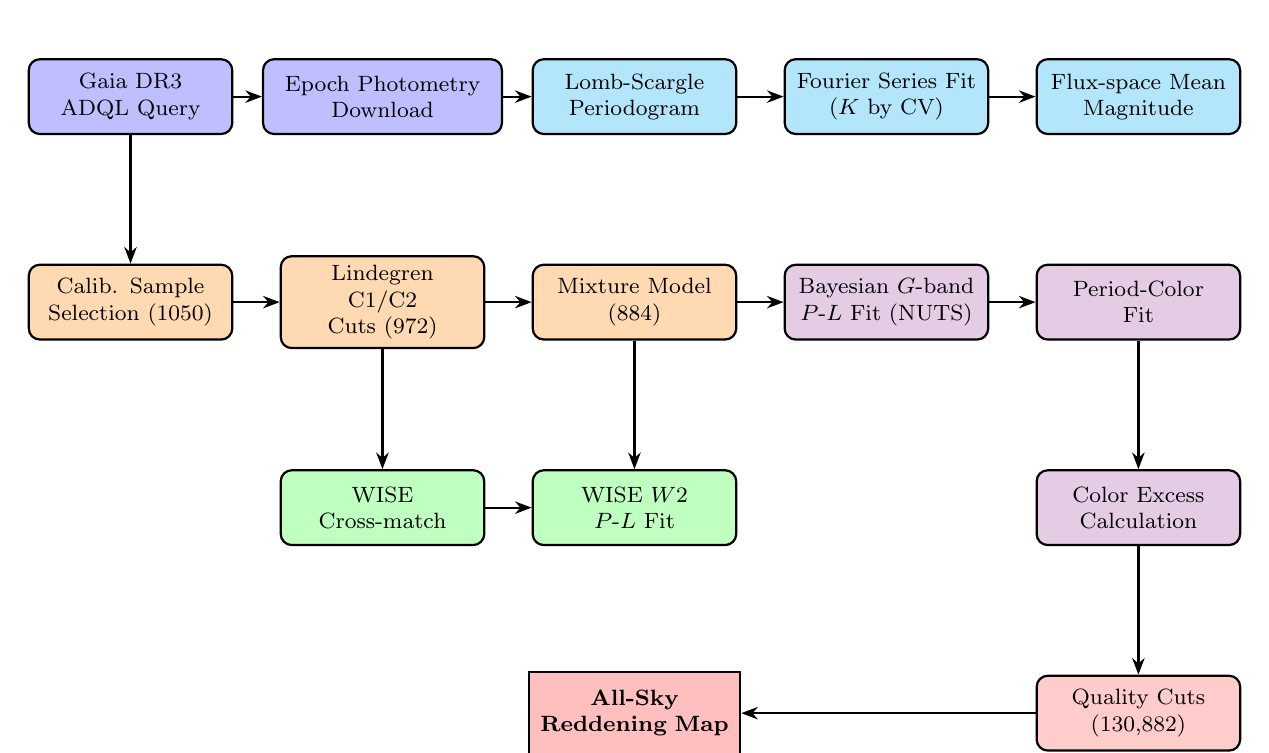
\begin{tikzpicture}[
    x=3.2cm,
    y=1.8cm,
    pipebox/.style={flowbox, text width=2.35cm, minimum height=0.95cm, font=\footnotesize},
    pipeout/.style={outputbox, text width=2.45cm, minimum height=1.05cm, font=\footnotesize},
  ]
    % Top row: data acquisition (blue) and light-curve processing (cyan)
    \node[pipebox, fill=blue!25] (gaia_adql) at (0,0) {Gaia DR3\\ADQL Query};
    \node[pipebox, fill=blue!25, text width=2.8cm] (lc_download) at (1,0) {Epoch Photometry\\Download};
    \node[pipebox, fill=cyan!30] (ls_period) at (2,0) {Lomb-Scargle\\Periodogram};
    \node[pipebox, fill=cyan!30] (fourier_fit) at (3,0) {Fourier Series Fit\\($K$ by CV)};
    \node[pipebox, fill=cyan!30] (mean_mag) at (4,0) {Flux-space Mean\\Magnitude};

    % Middle row: calibration (orange) and optical fits (violet)
    \node[pipebox, fill=orange!30] (calib_select) at (0,-1.45) {Calib. Sample\\Selection (1050)};
    \node[pipebox, fill=orange!30] (c1c2_cuts) at (1,-1.45) {Lindegren\\C1/C2 Cuts (972)};
    \node[pipebox, fill=orange!30] (mixture_model) at (2,-1.45) {Mixture Model\\(884)};
    \node[pipebox, fill=violet!20] (mcmc_pl) at (3,-1.45) {Bayesian $G$-band\\$P$-$L$ Fit (NUTS)};
    \node[pipebox, fill=violet!20] (pc_fit) at (4,-1.45) {Period-Color\\Fit};

    % Third row: infrared branch (green) and color excess (violet) dropping from pc_fit
    \node[pipebox, fill=green!25] (wise_xmatch) at (1,-2.9) {WISE\\Cross-match};
    \node[pipebox, fill=green!25] (wise_pl) at (2,-2.9) {WISE $W2$\\$P$-$L$ Fit};
    \node[pipebox, fill=violet!20] (color_excess) at (4,-2.9) {Color Excess\\Calculation};

    % Bottom row: dust map (red)
    \node[pipeout, fill=red!25] (sky_map) at (2,-4.35) {\textbf{All-Sky\\Reddening Map}};
    \node[pipebox, fill=red!20] (quality_cuts) at (4,-4.35) {Quality Cuts\\(130,882)};

    % Data and light-curve branch
    \draw[arrow] (gaia_adql) -- (lc_download);
    \draw[arrow] (lc_download) -- (ls_period);
    \draw[arrow] (ls_period) -- (fourier_fit);
    \draw[arrow] (fourier_fit) -- (mean_mag);

    % Calibration and optical fitting branch
    \draw[arrow] (gaia_adql) -- (calib_select);
    \draw[arrow] (calib_select) -- (c1c2_cuts);
    \draw[arrow] (c1c2_cuts) -- (mixture_model);
    \draw[arrow] (mixture_model) -- (mcmc_pl);
    \draw[arrow] (mcmc_pl) -- (pc_fit);

    % Optical fits flowing down then left to dust map
    \draw[arrow] (pc_fit) -- (color_excess);
    \draw[arrow] (color_excess) -- (quality_cuts);
    \draw[arrow] (quality_cuts) -- (sky_map);

    % Infrared branch
    \draw[arrow] (c1c2_cuts.south) -- (wise_xmatch.north);
    \draw[arrow] (wise_xmatch) -- (wise_pl);
    \draw[arrow] (mixture_model.south) -- (wise_pl.north);
  \end{tikzpicture}%
  }
  \caption{Complete analysis pipeline from Gaia DR3 data acquisition to all-sky reddening map. Node color indicates pipeline stage: \textcolor{blue!70!black}{Data Access} (Gaia DR3 query and epoch photometry download); \textcolor{cyan!60!black}{Light Curves} (Lomb-Scargle periodogram, Fourier series fitting, flux-space mean magnitude); \textcolor{orange!70!black}{Calibration} (sample selection and astrometric quality cuts); \textcolor{violet}{Optical Fits} (Bayesian $G$-band $P$-$L$ fit, period-color relation, color excess); \textcolor{green!60!black}{Infrared Branch} (WISE cross-match and $W2$ $P$-$L$ fit); \textcolor{red!60!black}{Dust Map} (quality filtering and all-sky reddening map).}
  \label{fig:pipeline}
\end{figure*}

%%% ---------------------------------------------------------------
\section{Theoretical Background}
\label{sec:theory}
%%% ---------------------------------------------------------------

\subsection{RR Lyrae Pulsation}

RR Lyrae stars are low-mass ($\sim 0.6\,M_\odot$), metal-poor, evolved stars on the horizontal branch (HB). After exhausting core hydrogen on the main sequence, these stars settled on the HB with helium-burning cores. Those HB stars that fall within the classical instability strip in the Hertzsprung-Russell diagram undergo radial pulsations driven by the $\kappa$-mechanism \citep{CatelanSmith2015}.

RR Lyrae stars are classified by their pulsation mode:
\begin{itemize}
  \item \textbf{RRab}: fundamental-mode pulsators with periods $P \approx 0.3$--1.0 days, characterized by large amplitudes ($\Delta G \sim 0.5$--1.5 mag) and asymmetric, sawtooth-shaped light curves with a rapid rise and slower decline.
  \item \textbf{RRc}: first-overtone pulsators with shorter periods ($P \approx 0.2$--0.4 days), smaller amplitudes ($\Delta G \sim 0.2$--0.5 mag), and more sinusoidal light curves.
  \item \textbf{RRd}: double-mode pulsators exciting both fundamental and first-overtone modes simultaneously; much rarer.
\end{itemize}

The Blazhko effect refers to the observed quasi-periodic modulations of the light curve amplitude and phase on timescales of tens to hundreds of days \citep{Netzel2018}. Stars exhibiting the Blazhko effect show residuals from simple periodic models, complicating period determination. 

\subsection{Period-Luminosity Relations}

The Leavitt law \citep{Leavitt1912} for classical Cepheids demonstrated that pulsation period correlates with intrinsic luminosity. RR Lyrae stars follow an analogous but weaker period-luminosity relation \citep{CatelanSmith2015}:
\begin{equation}
  M_\lambda = a_\lambda \log P + b_\lambda + Z_\lambda [\mathrm{Fe/H}],
\end{equation}
where $M_\lambda$ is absolute magnitude in band $\lambda$, $P$ is the pulsation period, and $[\mathrm{Fe/H}]$ is metallicity. The metallicity dependence $Z_\lambda$ is significant in optical bands (e.g. Gaia band $G$) but diminishes in the infrared (e.g. WISE band $W2$).

Notably, PL relations have wavelength dependence whereby slopes are steeper and scatter is smaller in the infrared. This is because dust extinction decreases with wavelength ($A_\lambda \propto \lambda^{-\alpha}$, $\alpha \sim 1.7$), so infrared PL relations are less sensitive to residual extinction in the calibration sample. WISE band $W2$ (4.6 $\mu$m) offers the additional advantage that the $R_{W2}$ extinction coefficient is nearly negligible \citep{KleinBloom2014}.

\subsection{Lomb-Scargle Periodogram}

Gaia light curves are irregularly sampled due to the satellite's observation strategy. The standard Fourier transform assumes uniform sampling, so we use the Lomb-Scargle (LS) periodogram \citep{Lomb1976, Scargle1982}, which generalizes frequency analysis to unevenly sampled data.

For a time series $\{t_i, y_i, \sigma_i\}$, the LS periodogram is defined as \citep{VanderPlas2018}:
\begin{equation}
  \begin{split}
    P_{\rm LS}(\omega) = \frac{1}{2\hat{\chi}^2} \Biggl[
      \frac{\left(\sum_i w_i y_i \cos\omega(t_i - \tau)\right)^2}{\sum_i w_i \cos^2\omega(t_i-\tau)} \\
      \qquad + \frac{\left(\sum_i w_i y_i \sin\omega(t_i - \tau)\right)^2}{\sum_i w_i \sin^2\omega(t_i-\tau)}
    \Biggr],
  \end{split}
\end{equation}
where $w_i \propto \sigma_i^{-2}$ are measurement weights, $\hat{\chi}^2$ is the weighted variance of the data, and $\tau$ is a phase offset chosen to orthogonalize the sine and cosine terms. The LS power $P_{\rm LS}(\omega) \in [0, 1]$ measures the fraction of variance explained by a sinusoid at angular frequency $\omega = 2\pi/P$. The period estimate is the frequency at maximum power.

False alarm probabilities (FAPs) quantify the significance of peaks against noise fluctuations. For the datasets considered here (Gaia light curves with $\sim$30--100 epochs), the highest LS peak is typically highly significant ($\mathrm{FAP} \ll 10^{-10}$).

\subsection{Fourier Series Modeling}

A single sinusoid often poorly fits RR Lyrae light curves, particularly for RRab stars. Hence, we model the light curve as a truncated Fourier series of order $K$:
\begin{equation}
  G(\phi) = A_0 + \sum_{k=1}^{K} \left[ A_k \cos(2\pi k \phi) + B_k \sin(2\pi k \phi) \right],
\end{equation}
where $\phi = (t - t_0)/P \bmod 1$ is the pulsation phase. This can be written in matrix form as $\mathbf{G} = \mathbf{X}\boldsymbol{\beta}$, where the design matrix $\mathbf{X}$ has rows:
\begin{equation}
  \begin{split}
    \mathbf{x}_i = \bigl[ 1,\, \cos(2\pi\phi_i),\, \sin(2\pi\phi_i),\, \ldots,\, \\
      \cos(2\pi K\phi_i),\, \sin(2\pi K\phi_i) \bigr].
  \end{split}
\end{equation}
The least-squares solution is $\hat{\boldsymbol{\beta}} = (\mathbf{X}^T \mathbf{W} \mathbf{X})^{-1} \mathbf{X}^T \mathbf{W} \mathbf{G}$, where $\mathbf{W} = \mathrm{diag}(\sigma_i^{-2})$.

The per-epoch weights $\sigma_{G,i}$ combine the Gaia epoch flux signal-to-noise and the $G$-band zero-point uncertainty $\sigma_{\rm ZP}$:
\begin{equation}
  \sigma_{G,i} = \sqrt{\left(\frac{2.5}{\ln 10}\,\frac{\sigma_{f,i}}{f_i}\right)^{\!2} + \sigma_{\rm ZP}^2}. \label{eq:sigma_G}
\end{equation}
The formal coefficient covariance is:
\begin{equation}
  C_{\boldsymbol{\beta}} = \max\!\left(\chi_\nu^2,\,1\right)(\mathbf{X}^T\mathbf{W}\mathbf{X})^{-1},
\end{equation}
where $\chi_\nu^2 = (N - 2K - 1)^{-1}\sum_i (G_i - \hat{G}_i)^2/\sigma_{G,i}^2$. All downstream Fourier uncertainties (predicted magnitudes, mean magnitude) are propagated from $C_{\boldsymbol{\beta}}$.

The order $K$ is chosen by cross-validation (CV) where we split the light curve into training ($\sim$80\%) and validation ($\sim$20\%) sets, fit on the training set for each $K$, and select the $K$ that minimizes the validation reduced $\chi^2_r$:
\begin{equation}
  \chi^2_r = \frac{1}{N_{\rm CV}} \sum_{i \in \rm CV} \frac{(G_i - \hat{G}_i)^2}{\sigma_{G,i}^2}.
\end{equation}

The mean magnitude of the star is computed in two ways. The first is the epoch mean $\langle G \rangle_{\rm epoch}$, obtained by averaging the epoch fluxes and converting back to magnitudes:
\begin{equation}
  \langle G \rangle_{\rm epoch} = -2.5\log_{10}\!\left(\frac{1}{N}\sum_{i=1}^{N} f_i\right) + ZP_G,
\end{equation}
where $f_i$ are the Gaia epoch fluxes (\texttt{g\_transit\_flux}) and $ZP_G$ is the $G$-band zero-point.
The second is the Fourier mean $\langle G \rangle_{\rm Fourier}$, computed in flux space to avoid the non-linearity of the magnitude scale:
\begin{equation}
  \langle G \rangle_{\rm Fourier} = -2.5 \log_{10}\left[ \frac{1}{2\pi} \int_0^{2\pi} 10^{-0.4\, G(\phi)}\, d\phi \right].
\end{equation}
This integral is evaluated numerically from the Fourier fit coefficients, and its uncertainty is propagated from $C_{\boldsymbol{\beta}}$ by linearising $\langle G \rangle_{\rm Fourier}$ around $\hat{\boldsymbol{\beta}}$ and $\sigma_{\langle G \rangle}^2 \approx (\nabla_{\boldsymbol{\beta}} \langle G \rangle)^T C_{\boldsymbol{\beta}}\, (\nabla_{\boldsymbol{\beta}} \langle G \rangle)$, with the gradient evaluated numerically over a phase grid.

\subsection{Bayesian MCMC Inference}

We fit the PL relation using Bayesian inference. The posterior distribution over parameters $\boldsymbol{\theta} = (a, b, \sigma_{\rm scatter})$ is:
\begin{equation}
  p(\boldsymbol{\theta} \mid \mathbf{y}) \propto p(\mathbf{y} \mid \boldsymbol{\theta})\, p(\boldsymbol{\theta}),
\end{equation}
where $p(\mathbf{y} \mid \boldsymbol{\theta})$ is the likelihood and $p(\boldsymbol{\theta})$ the prior.

The likelihood accounts for both measurement uncertainties $\sigma_i$ and intrinsic astrophysical scatter $\sigma_{\rm scatter}$ (due to metallicity spread, depth effects, etc.). Defining $\delta_i \equiv \log P_i - \langle\log P\rangle_{\rm class}$ as the centered log-period:
\begin{equation}
  \begin{split}
    \log\mathcal{L} = -\frac{1}{2} \sum_i \left[
      \frac{(M_{G,i} - a\,\delta_i - b)^2}{\sigma_i^2 + \sigma_{\rm scatter}^2 + a^2\sigma_{\log P,i}^2} \right. \\
      \left. + \log(2\pi(\sigma_i^2 + \sigma_{\rm scatter}^2 + a^2\sigma_{\log P,i}^2)) \right].
  \end{split}
\end{equation}
Here $\sigma_{M,i}^2 = \sigma_{G,i}^2 + \sigma_{\mu,i}^2$ combines the apparent-magnitude and distance-modulus uncertainties in quadrature. The apparent-magnitude error follows the same form as Eq.~\eqref{eq:sigma_G}, with $f_i$ and $\sigma_{f,i}$ replaced by the catalog mean flux $F_i$ (\texttt{phot\_g\_mean\_flux}) and its uncertainty $\sigma_{F,i}$ (\texttt{phot\_g\_mean\_flux\_error}). The distance-modulus error propagates the Gaia parallax uncertainty $\sigma_{\varpi,i}$:
\begin{equation}
  \sigma_{\mu,i} = \frac{5\,\sigma_{\varpi,i}}{\varpi_i \ln 10}.
\end{equation}

We implement three MCMC samplers:

\textbf{Metropolis-Hastings (M-H):} A random-walk sampler that proposes steps $\boldsymbol{\theta}' = \boldsymbol{\theta} + \boldsymbol{\epsilon}$, $\boldsymbol{\epsilon} \sim \mathcal{N}(\mathbf{0}, \boldsymbol{\Sigma}_{\rm prop})$, and accepts with probability $\alpha = \min(1, p(\boldsymbol{\theta}')/p(\boldsymbol{\theta}))$ \citep{Metropolis1953, Hastings1970}. The per-parameter proposal standard deviations are tuned by scanning a discrete grid and selecting the scale whose acceptance rate is closest to $\sim$0.5.

\textbf{NUTS (No-U-Turn Sampler):} A Hamiltonian Monte Carlo (HMC) variant \citep{HoffmanGelman2014}. HMC augments the parameter vector $\boldsymbol{\theta}$ with auxiliary momentum variables $\mathbf{p}$ and simulates Hamiltonian dynamics along the posterior surface whereby the gradient $\nabla\log p(\boldsymbol{\theta}\mid\mathbf{y})$ acts as a force that propels the sampler along high-probability regions, allowing large, nearly uncorrelated steps rather than the local random-walk steps of M-H. NUTS extends HMC by automatically determining how long to run each trajectory where it doubles the path length until the trajectory would start turning back on itself, after which it selects a point from the completed trajectory. Additionally, step sizes are automatically selected during the warm-up phase, removing the manual proposal-width grid search required by M-H. We implement NUTS both with a custom \texttt{Potential} term in PyMC and using native PyMC distributions.

\subsection{Interstellar Extinction via Period-Color Residuals}

Interstellar dust reddens starlight by absorbing and scattering photons. The color excess $E(G_{\rm BP} - G_{\rm RP})$ describes the difference between observed and intrinsic color:
\begin{align}
  E(G_{\rm BP} - G_{\rm RP}) &= (G_{\rm BP} - G_{\rm RP})_{\rm obs} \notag \\
                              &\quad - (G_{\rm BP} - G_{\rm RP})_{\rm int}(P),
\end{align}
where the intrinsic color $(G_{\rm BP} - G_{\rm RP})_{\rm int}(P)$ is predicted from our class-specific period-color calibration (Section~\ref{sec:data}).

The $G$-band extinction is then:
\begin{equation}
  A_G = R_G \cdot E(G_{\rm BP} - G_{\rm RP}),
\end{equation}
where $R_G = 2.0$ is the ratio of total-to-selective extinction adopted for the Gaia $G$ band. This value is consistent with the extinction law of \citet{Cardelli1989} as updated by \citet{ODonnell1994} applied to the Gaia $G$ bandpass, and with the empirical calibration by \citet{WangChen2019} who find $R_G \approx 2.0$ for Gaia DR2 photometry at typical red giant temperatures. Conceptually, since the Gaia DR3 $G$ band is broad, and $R_G$ has mild color dependence, for the range of stellar temperatures relevant to RR Lyrae ($T_{\rm eff} \sim 6000$--7500 K), $R_G \approx 2.0$ is an appropriate approximation.

%%% ---------------------------------------------------------------
\section{Data Acquisition}
\label{sec:data}
%%% ---------------------------------------------------------------

\subsection{Gaia DR3 Light Curve Sample (100 Stars)}

We began by querying the Gaia DR3 \texttt{vari\_rrlyrae} catalog for 100 high-quality RR Lyrae stars suitable for light curve analysis. The selection prioritized high-epoch-count stars for reliable period recovery:
\begin{itemize}
  \item \texttt{pf IS NOT NULL} (defined fundamental period)
  \item \texttt{num\_clean\_epochs\_g} $> 40$ (high epoch count for period recovery)
  \item Ordered by \texttt{num\_clean\_epochs\_g DESC}, limiting to 100 stars
\end{itemize}
The query was submitted via the Gaia TAP service using \texttt{astroquery.gaia}. Epoch photometry (time, magnitude, flux, uncertainty) for each star was then downloaded individually from the Gaia epoch photometry tables.

\subsection{Calibration Sample (1050 Stars)}

For the period-luminosity calibration, we required a sample of nearby, low-extinction RR Lyrae stars with precise Gaia parallaxes. The calibration sample was selected with:
\begin{itemize}
  \item \texttt{parallax\_over\_error} $> 5$ (relative parallax error $< 20\%$)
  \item $|b| > 30^\circ$ (high Galactic latitude, low extinction)
  \item Distance $d < 4$ kpc (derived from $\varpi > 0.25$ mas)
\end{itemize}
This returned 1050 stars with sufficient data for Bayesian PL fitting.

\subsection{Full All-Sky Catalog (269,772 Stars)}

For dust mapping, we downloaded the complete Gaia DR3 RR Lyrae catalog without distance restrictions. This returned 269,772 stars, forming the basis for the all-sky reddening map.

\subsection{WISE W2 Cross-Match}

Infrared photometry in WISE $W2$ (4.6 $\mu$m) was retrieved for calibration sample stars via the Gaia DR3 \texttt{allwise\_best\_neighbour} table. This cross-match links Gaia sources to their nearest AllWISE counterpart within a 1 arcsec radius. Referemce Gaia DR3 stars were required to have a unique best WISE neighbour, finite $W2$ magnitude and uncertainty, photometric quality flag \texttt{ph\_qual[1]} of \texttt{A} or \texttt{B}, no contamination flag (\texttt{cc\_flags[1] = '0'}), and no extended-source flag (\texttt{ext\_flag} $\leq 1$).

%%% ---------------------------------------------------------------
\section{Light Curve Analysis}
\label{sec:lc}
%%% ---------------------------------------------------------------

Throughout this section we use Gaia DR3 source \texttt{4659759557323962752} as a running example to illustrate each analysis step.

\subsection{Period Recovery via Lomb-Scargle}

We applied the Lomb-Scargle periodogram to the $G$-band epoch photometry of each of the 100 sample stars. The peak frequency $\omega_{\rm max}$ was identified, and the period $P_{\rm LS} = 2\pi/\omega_{\rm max}$ was recorded.

Figure~\ref{fig:lc_raw_phased} shows raw and phase-folded light curves for an example RRab star, and Figure~\ref{fig:periodogram} shows the corresponding LS periodogram.

\begin{figure*}[t]
  \centering
  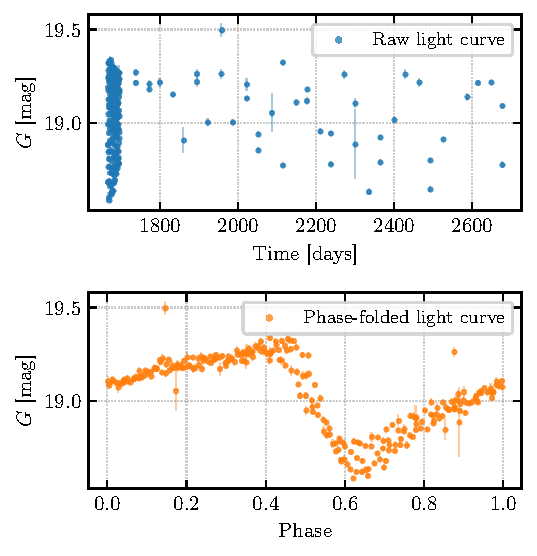
\includegraphics[width=\textwidth]{figures/fig_lc_raw_phased.pdf}
  \caption{Example Gaia DR3 $G$-band light curve for an RRab star. \textit{Left:} Raw time series with photometric uncertainties. \textit{Right:} Phase-folded light curve using the LS-recovered period, showing the characteristic sawtooth morphology of fundamental-mode pulsation.}
  \label{fig:lc_raw_phased}
\end{figure*}

\begin{figure}[H]
  \centering
  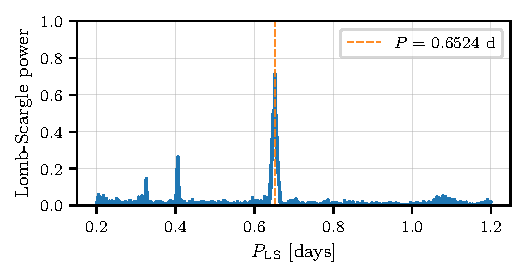
\includegraphics[width=\columnwidth]{figures/fig_periodogram.pdf}
  \caption{Lomb-Scargle periodogram for the star shown in Figure~\ref{fig:lc_raw_phased}. The vertical dashed line marks the peak period $P_{\rm LS}$ adopted for subsequent Fourier fitting.}
  \label{fig:periodogram}
\end{figure}

\subsubsection{Period Comparison with Gaia Catalog}

Figure~\ref{fig:period_comparison} compares our recovered periods to the Gaia DR3 catalog fundamental periods (\texttt{pf}). We find that 89 of 100 stars agree to within 1\% ($|P_{\rm LS} - P_{\rm pf}|/P_{\rm pf} < 0.01$). For all 11 outlying stars, inspection of the LS power spectrum reveals a second significant peak at a longer period agreeing to \texttt{pf}; the recovered $P_{\rm LS}$ matches the Gaia first-overtone period \texttt{p1o} rather than the fundamental \texttt{pf}. This identifies them as RRd double-mode pulsators, whose light curves contain power at both $P_0$ (fundamental) and $P_1$ (first overtone, $P_1/P_0 \approx 0.745$). The LS periodogram latches onto whichever peak carries the most power, which for these stars is $P_1$.

In the phase-folded light curves of several stars in the sample, low-amplitude quasi-periodic modulations characteristic of the Blazhko effect are visible as a scatter that is coherent on long timescales but incoherent within a single epoch window. However, the LS power associated with the Blazhko side-lobes (typically $\Delta\nu \sim 1/P_{\rm Blazhko}$ away from the main peak) is orders of magnitude smaller than the main pulsation peak. Consequently, the Blazhko effect does not displace the highest LS peak and has no effect on our period recovery; its likely only signature is a slight accentuation of the residuals after phase-folding on the recovered period.

\begin{figure*}[t]
  \centering
  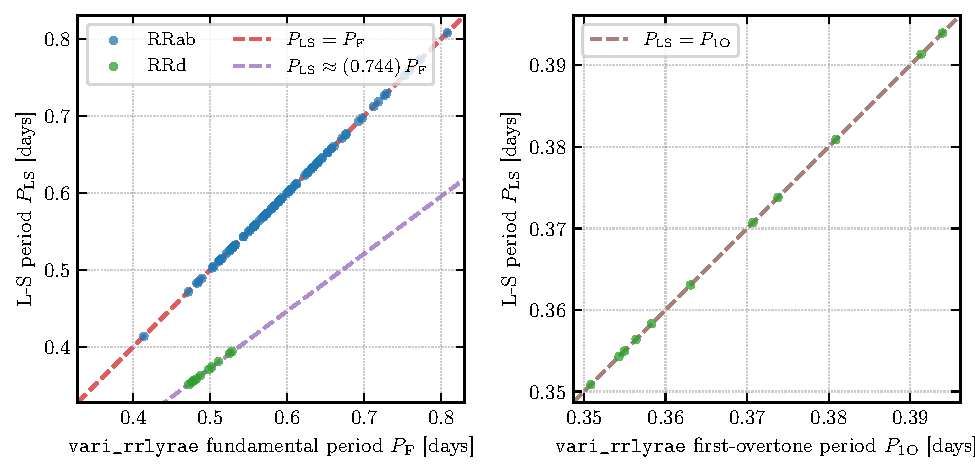
\includegraphics[width=\textwidth]{figures/fig_period_comparison.pdf}
  \caption{Comparison of LS-recovered periods to Gaia DR3 catalog fundamental periods (\texttt{pf}) for 100 stars. Points within 1\% agreement (89/100) are shown in blue; outlying stars are in red. The diagonal line shows perfect agreement. For all 11 red points, the recovered period matches the Gaia first-overtone period \texttt{p1o}, identifying them as RRd double-mode pulsators.}
  \label{fig:period_comparison}
\end{figure*}


\subsection{Fourier Series Fitting and Cross-Validation}

For each star, we fit Fourier series of orders $K = 1, 3, 5, 7, 9$ to the phase-folded light curve using weighted least squares. The design matrix $\mathbf{X}$ for each order was constructed as described in Section~\ref{sec:theory}. Figure~\ref{fig:fourier_harmonics} shows the progression of fit quality with increasing $K$ for the example star.

\begin{figure*}[p]
  \centering
  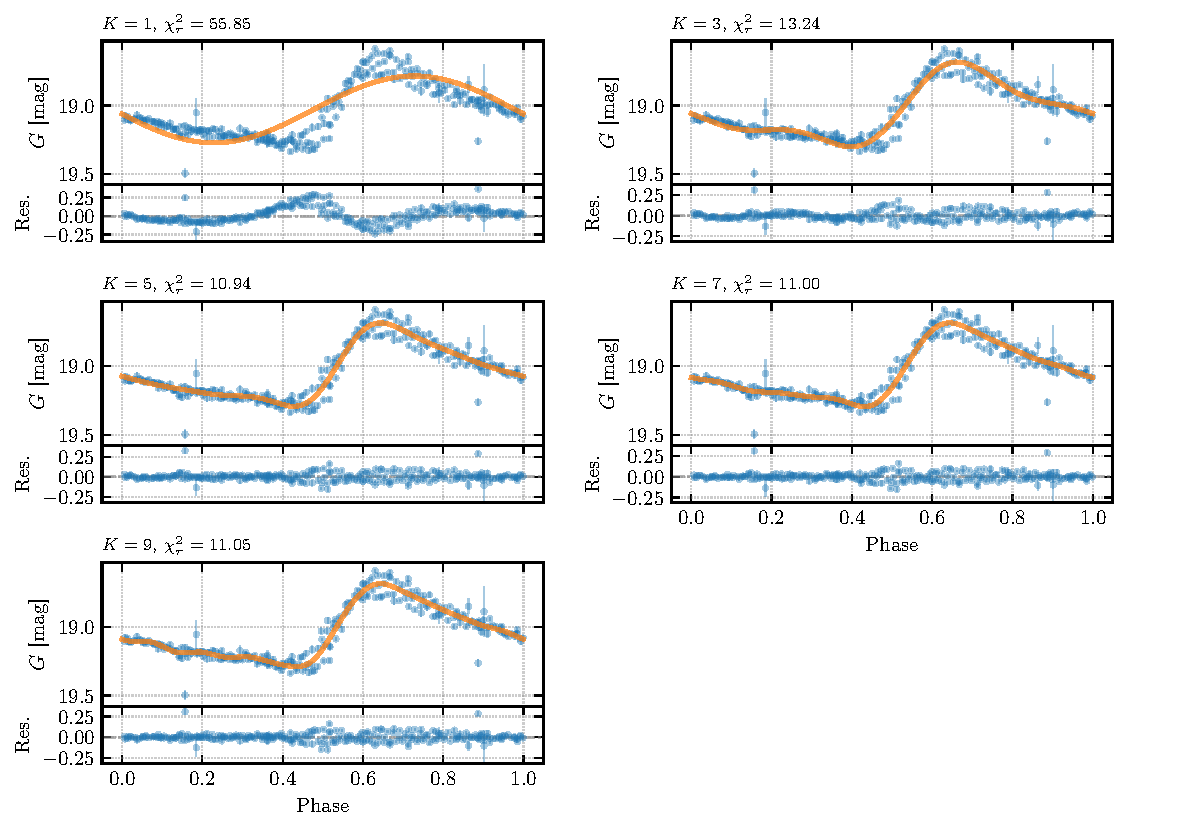
\includegraphics[width=\textwidth]{figures/fig_fourier_harmonics.pdf}
  \caption{Fourier series fits of order $K = 1, 3, 5, 7, 9$ to the phase-folded RRab light curve. Low orders ($K=1, 3$) fail to capture the rapid rise; $K=5$ provides a good fit; higher orders begin to overfit noise.}
  \label{fig:fourier_harmonics}
\end{figure*}

The optimal $K$ was selected via cross-validation (Figure~\ref{fig:crossval}). The training reduced $\chi^2_r$ monotonically decreases with $K$, while the validation $\chi^2_r$ has a minimum at $K \approx 5$--7 for most stars, beyond which overfitting to noise causes the validation error to increase. We adopted the $K$ minimizing validation $\chi^2_r$ for each star.

\begin{figure}[H]
  \centering
  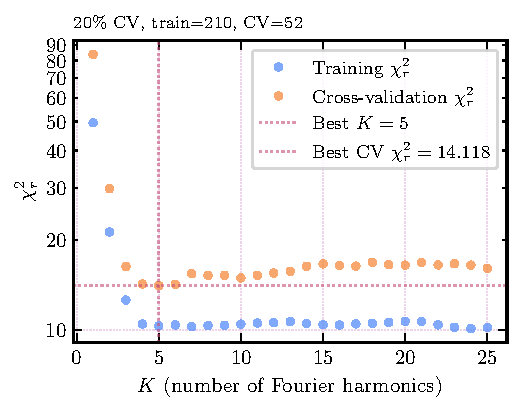
\includegraphics[width=\columnwidth]{figures/fig_crossval.pdf}
  \caption{Cross-validation curve for the example RRab star where training $\chi^2_r$ (blue) and validation $\chi^2_r$ (orange) as a function of Fourier order $K$. The optimal $K = 5$ minimizes validation error before overfitting sets in.}
  \label{fig:crossval}
\end{figure}

Figures~\ref{fig:cv_residuals} and \ref{fig:cv_phase} further diagnose the underfitting and overfitting regimes. Figure~\ref{fig:cv_residuals} shows normalised residuals $(G - G_{\rm model})/\sigma$ for the low-$K$ and best-$K$ fits on both the training and validation sets. In the low-$K$ panel both distributions are broader than the reference $\mathcal{N}(0,1)$, indicating genuine light-curve structure left in the residuals. At best $K$ the two distributions converge and narrow toward unity, showing the model now captures the dominant astrophysical shape. Figure~\ref{fig:cv_phase} compares the best-$K$ and high-$K$ phase fits. Here, the high-$K$ model interpolates training-set noise and departs from the validation points.

\begin{figure*}[t]
  \centering
  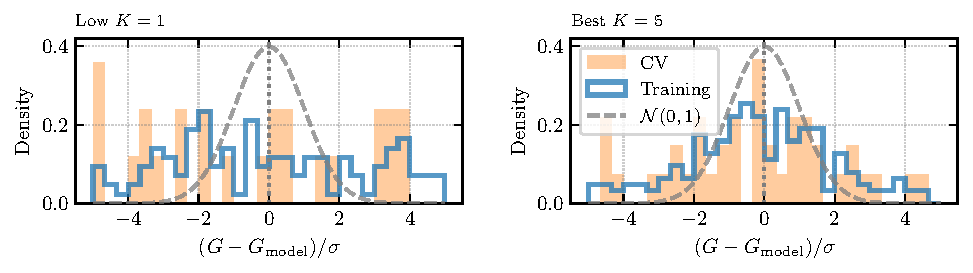
\includegraphics[width=\textwidth]{figures/fig_fourier_cv_residuals.pdf}
  \caption{Normalised residual histograms $(G - G_{\rm model})/\sigma$ for the training (blue outline) and validation (orange fill) sets. \textit{Left:} In the low-$K$ underfitting regime, both distributions are broader than $\mathcal{N}(0,1)$ (dashed), indicating unmodelled light-curve structure. \textit{Right:} In the best-$K$ regime, training and validation residuals converge and approach the reference Gaussian, showing adequate model complexity.}
  \label{fig:cv_residuals}
\end{figure*}

\begin{figure*}[b]
  \centering
  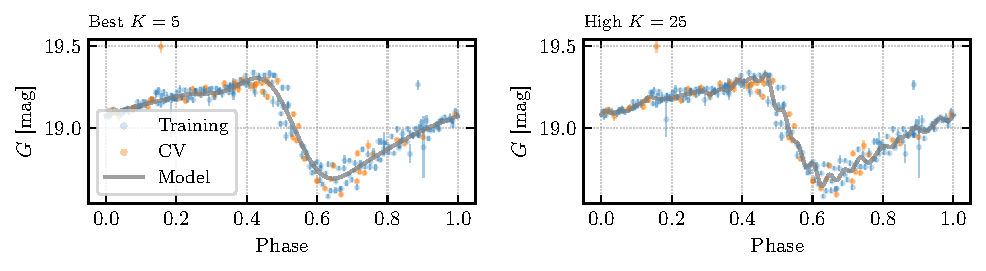
\includegraphics[width=\textwidth]{figures/fig_fourier_cv_phase.pdf}
  \caption{Phase-folded light curves for the best-$K$ (left) and high-$K$ (right) Fourier fits. Training epochs are shown in blue and validation epochs in orange. The high-$K$ model overfits training noise and diverges from the validation points.}
  \label{fig:cv_phase}
\end{figure*}

\subsection{Flux-Space Mean Magnitudes}

A key advantage of the Fourier model is accurate mean magnitude estimation. Averaging magnitudes directly is biased because the relationship between flux and magnitude is nonlinear ($f \propto 10^{-0.4m}$). We instead computed the mean flux from the Fourier model by numerical integration in flux space and converted back to magnitude (see Section~\ref{sec:theory}).

Figure~\ref{fig:mean_g_comparison} compares both estimators against the Gaia DR3 \texttt{int\_average\_g} (the catalog intensity-averaged magnitude). The left panel shows the flux-space epoch mean, $\langle G \rangle_{\rm epoch}$, against the catalog value; the right panel shows $\langle G \rangle_{\rm Fourier}$. Residual panels below each scatter plot show the signed offset from the catalog. The Fourier-based mean is more tightly clustered around the one-to-one line, with RMS residual 0.0147 mag vs.\ 0.0282 mag for the epoch mean. The improvement arises because the Fourier template reconstructs the full pulsation cycle, correcting for uneven phase sampling across Gaia visits that inflates the epoch-average scatter.

\begin{figure*}[t]
  \centering
  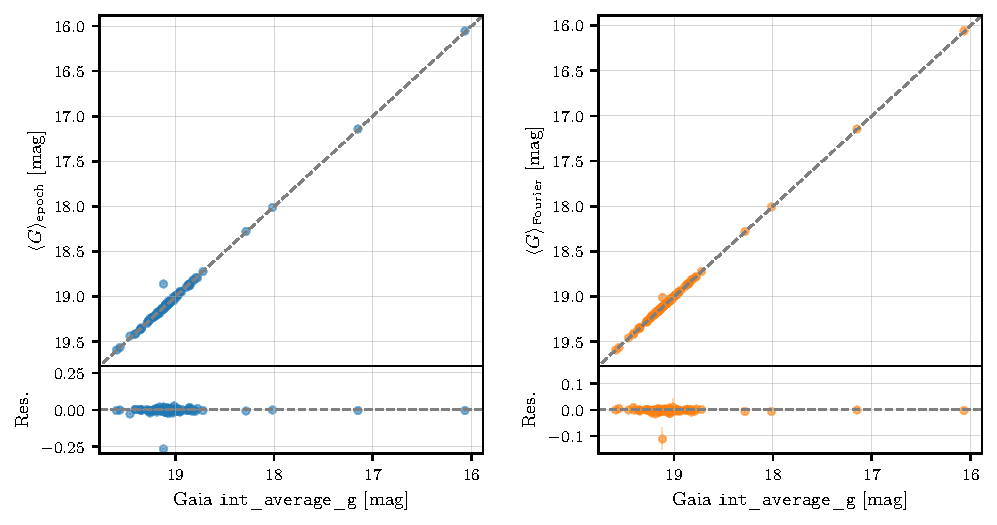
\includegraphics[width=\textwidth]{figures/fig_mean_g_comparison.pdf}
  \caption{Comparison of mean $G$-band magnitude estimators against the Gaia DR3 \texttt{int\_average\_g} catalog value. \textit{Left:} Flux-space epoch mean $\langle G \rangle_{\rm epoch}$ vs.\ catalog; \textit{Right:} Fourier mean $\langle G \rangle_{\rm Fourier}$ vs.\ catalog. Residual panels (bottom) show the signed offset; the dashed line marks zero. The Fourier mean achieves RMS $= 0.0147$ mag vs.\ $0.0282$ mag for the epoch mean.}
  \label{fig:mean_g_comparison}
\end{figure*}

\subsection{Light Curve Extrapolation}

The Fourier model, once fit, can predict the star's brightness at arbitrary future times. Figure~\ref{fig:fourier_extrapolation} shows a 10-day extrapolation beyond the last Gaia epoch for the running-example star. The shaded band represents the $\pm1\sigma$ predictive uncertainty propagated from the full Fourier coefficient covariance matrix $\mathbf{C}_\beta$; the vertical dashed line marks the last observed epoch.

\begin{figure*}[t]
  \centering
  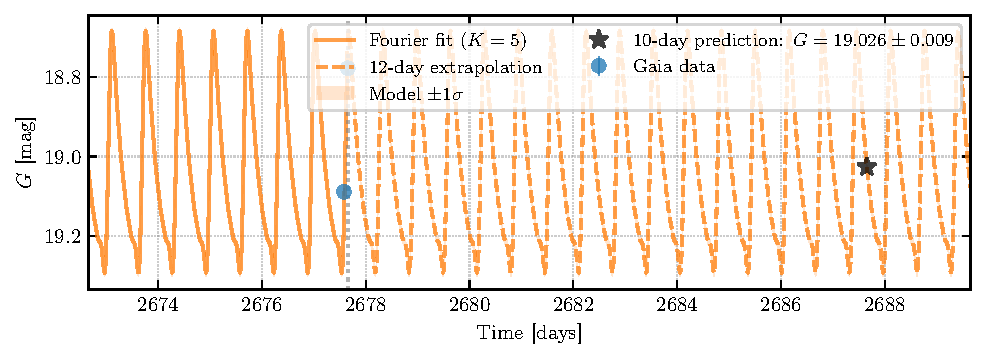
\includegraphics[width=\textwidth]{figures/fig_fourier_extrapolation.pdf}
  \caption{Light curve extrapolation for Gaia DR3 source \texttt{4659759557323962752}. The final five days of Gaia epoch photometry (grey points with error bars) anchor the best-fit Fourier model (orange curve). The shaded band shows the $\pm1\sigma$ uncertainty from the coefficient covariance $\mathbf{C}_\beta$. The vertical dashed line marks the last observed epoch; the model is extrapolated 10 days into the future.}
  \label{fig:fourier_extrapolation}
\end{figure*}

\subsection{RRab vs.\ RRc Morphology}

Figure~\ref{fig:rrab_rrc} illustrates the morphological differences between RRab and RRc light curves. RRab stars (left panels) show the characteristic sawtooth shape consisting of a rapid rise ($\sim$20\% of the period) followed by a slower decline, with peak-to-peak amplitudes of 0.5--1.5 mag in $G$. RRc stars (right panels) are more sinusoidal with smaller amplitudes (0.2--0.5 mag) and shorter periods. These differences reflect fundamentally different pulsation modes and instability strip locations \citep{CatelanSmith2015}.

\begin{figure*}[p]
  \centering
  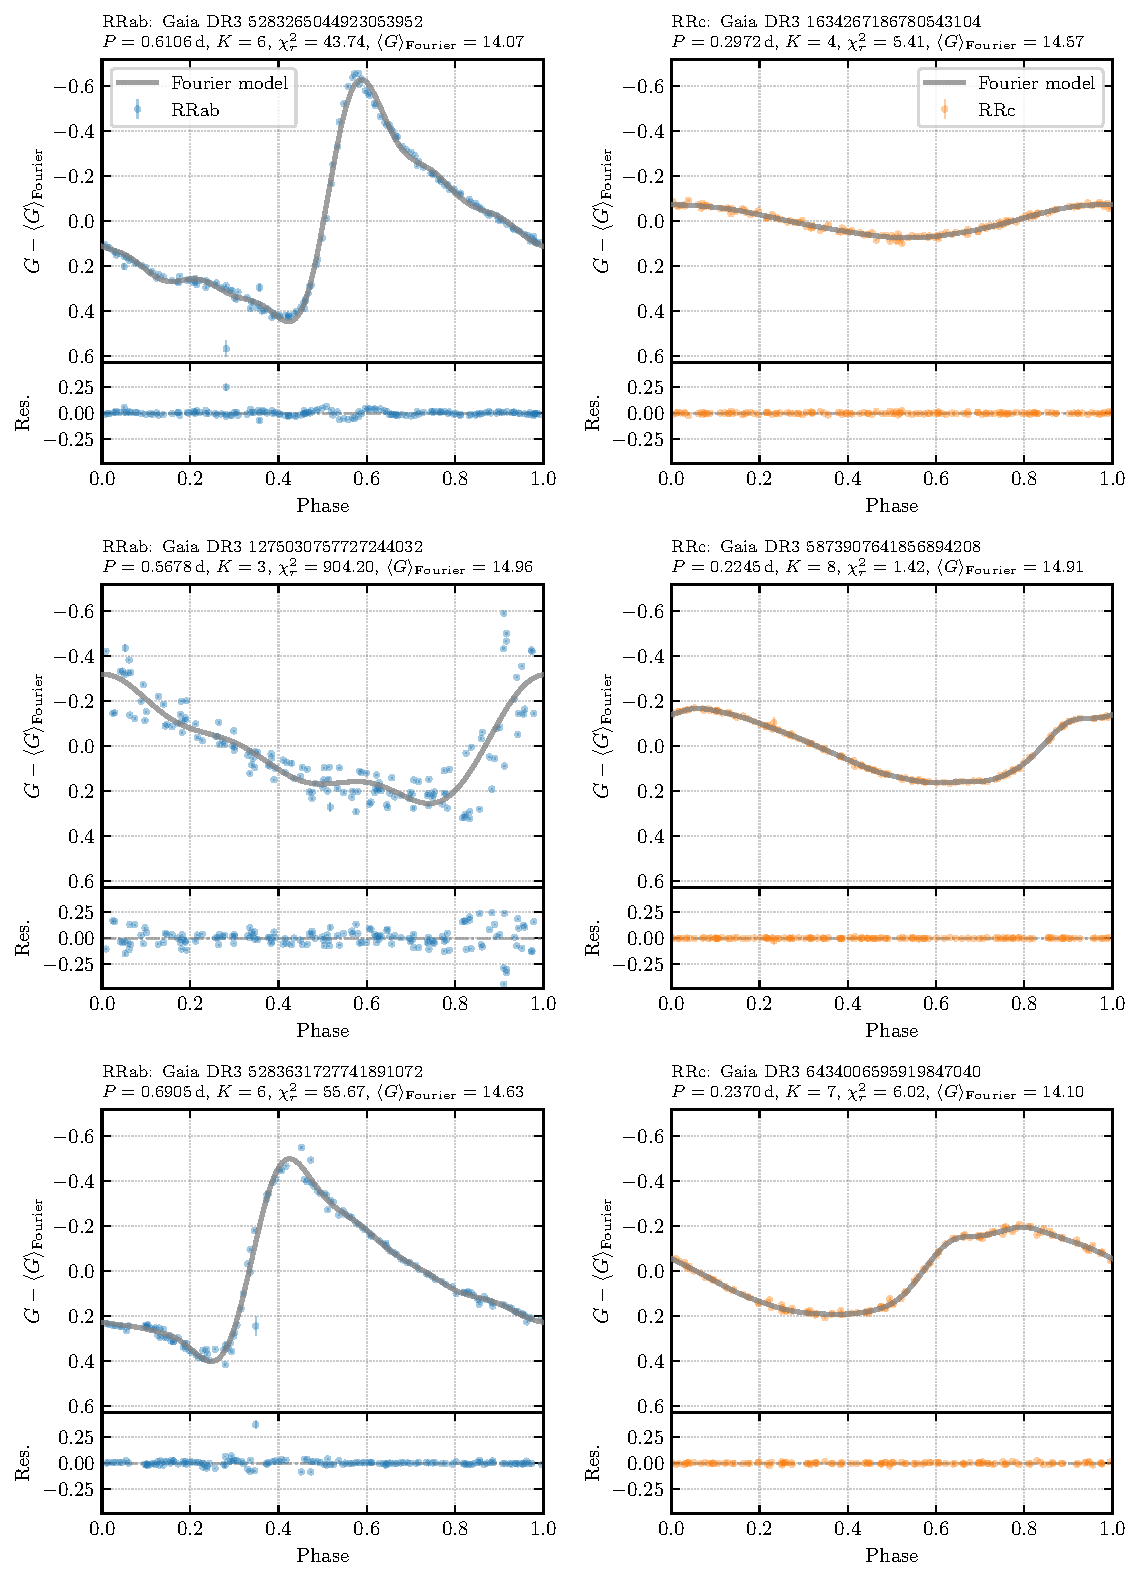
\includegraphics[width=\textwidth]{figures/fig_rrab_rrc.pdf}
  \caption{Representative phase-folded $G$-band light curves for three RRab (top) and three RRc (bottom) stars. RRab stars show large-amplitude, asymmetric sawtooth profiles typical of fundamental-mode pulsation; RRc stars are more sinusoidal with smaller amplitudes, consistent with first-overtone pulsation.}
  \label{fig:rrab_rrc}
\end{figure*}

%%% ---------------------------------------------------------------
\section{Calibration Sample Construction}
\label{sec:calib}
%%% ---------------------------------------------------------------

\subsection{Initial Selection}

The initial calibration sample of 1050 RR Lyrae stars (Section~\ref{sec:data}) spans the northern and southern sky at high Galactic latitudes. Figure~\ref{fig:calibration_sky_c12} shows the sky distribution in Aitoff projection; all stars lie outside the $|b| < 30^\circ$ exclusion zone by construction, confirming that the ADQL query has removed Galactic disk stars. The figure also shows the spatial pattern of stars removed versus retained after the C1/C2 cuts.

\subsection{Lindegren Astrometric Quality Cuts}

Raw parallaxes from Gaia DR3 can be affected by astrometric systematics, particularly for sources with poor five-parameter astrometric solutions. We applied two quality cuts following \citet{Lindegren2021}:

\textbf{C1 (astrometric unit-weight error):} We compute the astrometric unit-weight error $u = \sqrt{\chi^2_{\rm al}/(n_{\rm obs}-5)}$ from the along-scan $\chi^2$ and reject stars with $u > 1.2\max(1, e^{-0.2(G-19.5)})$. This magnitude-dependent threshold selects stars with well-behaved five-parameter astrometric solutions.

\textbf{C2 (BP/RP photometric excess):} Stars whose BP$+$RP excess factor $E$ falls outside the two-sided, colour-dependent envelope $1 + 0.015(G_{\rm BP}-G_{\rm RP})^2 < E < 1.3 + 0.06(G_{\rm BP}-G_{\rm RP})^2$ are flagged as likely blended or contaminated and removed.

After both cuts, the sample reduced from 1050 to 972 stars, a $\sim$7.4\% rejection rate. Of the 1050 stars, 1006 pass C1 alone and 973 pass C2 alone; only the 972 passing both cuts are retained. Table~\ref{tab:sample_cuts} summarizes the sample evolution through each cleaning stage.

An interesting feature of the removals is their spatial non-uniformity (Figure~\ref{fig:calibration_sky_c12}). The most conspicuous concentrations of rejected stars coincide with the directions of the Large and Small Magellanic Clouds (LMC and SMC), where crowding and source blending degrade Gaia's astrometric and photometric quality diagnostics. Because the sample already requires $\varpi > 0.25$\,mas, genuine Magellanic Cloud members at $\sim$50--60\,kpc are excluded by the parallax selection; the rejected clumps therefore represent problematic Gaia solutions projected against the Cloud directions, not actual Cloud members. This makes their removal by C1/C2 physically sensible. Quantitatively, among the 78 stars removed by C1/C2, those within $10^\circ$ of the LMC center have a rejection rate of 3/24 = 12.5\%, while those within $6^\circ$ of the SMC center show a strikingly high rejection rate of 19/24 = 79.2\%. By contrast, stars elsewhere on the sky are removed at only 56/945 = 5.9\%, the expected baseline rate driven by genuine astrometric outliers. The 79\% rejection fraction toward the SMC provides strong empirical evidence that crowding-induced catalog artifacts are highly concentrated in that direction.

\begin{figure*}[t]
  \centering
  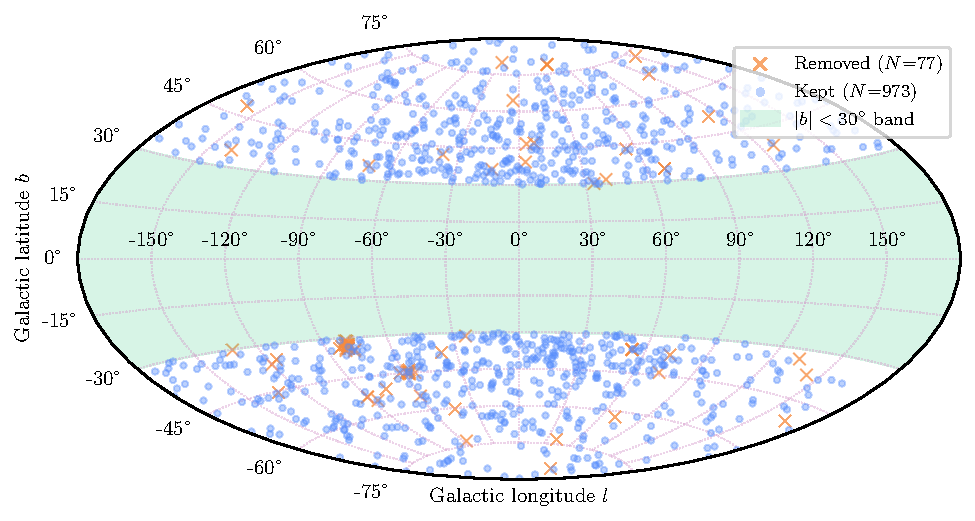
\includegraphics[width=\textwidth]{figures/fig_calibration_sky_c12.pdf}
  \caption{Stars removed (orange) versus retained (blue) after the Lindegren C1/C2 quality cuts. Rejected stars cluster toward the LMC ($l \approx 280^\circ$, $b \approx -33^\circ$) and SMC ($l \approx 303^\circ$, $b \approx -44^\circ$) directions, where crowding degrades Gaia astrometric and photometric solutions. These are not Magellanic Cloud members (since the $\varpi > 0.25$\,mas cut already excludes stars beyond 4\,kpc) but rather problematic catalog solutions in crowded fields.}
  \label{fig:calibration_sky_c12}
\end{figure*}

\subsection{Mixture Contamination Model}

Even after astrometric quality cuts, some outliers remain in the PL plane. These may be genuinely misclassified stars, unresolved binaries affecting the parallax, or stars with anomalous extinction. We modeled the data as a mixture of two populations \citep{Hogg2010}:
\begin{itemize}
  \item \textbf{Inliers} ($f_{\rm in}$): true RR Lyrae stars following the PL relation, with residuals $\epsilon_i \sim \mathcal{N}(0, \sigma_i^2 + \sigma_{\rm int}^2)$.
  \item \textbf{Outliers} ($1-f_{\rm in}$): contaminating sources with large, uninformative scatter $\sigma_{\rm out} \gg \sigma_{\rm int}$.
\end{itemize}

The mixture likelihood for star $i$ is:
\begin{multline}
  p(M_i \mid \boldsymbol{\theta}) = f_{\rm in}\, \mathcal{N}(M_i;\, a\,\delta_i + b,\, \sigma_i^2 + \sigma_{\rm int}^2) \\
    + (1-f_{\rm in})\, \mathcal{N}(M_i;\, \mu_{\rm out},\, \sigma_{\rm out}^2).
\end{multline}
Each star's posterior inlier probability $p_{{\rm in},i}$ is computed from the ratio of likelihood components. Stars with $p_{{\rm in},i} < 0.95$ were removed, reducing the sample from 972 to 884 stars. Figure~\ref{fig:pl_stages} shows the PL relation before and after C1/C2 cuts, and Figure~\ref{fig:pl_inlier} shows the mixture-model inlier probabilities and the final cleaned sample.

The progressive improvement can also in quantified in scatter. The largest improvement occurs at the mixture model step where the RMS falls from 1.229 to 0.259 mag (a further 79\% reduction), and the number of stars more than 1 mag from the relation drops from 48 to just 1. The C1/C2 cuts alone provide a 57\% RMS improvement, primarily by removing the long tails in the parallax error distribution.

\begin{figure}[H]
  \centering
  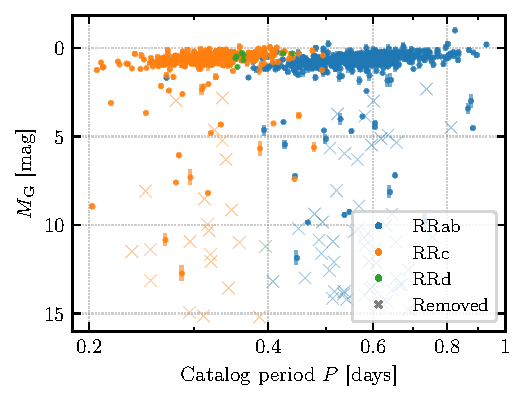
\includegraphics[width=\columnwidth]{figures/fig_period_abs_mag_c12_comparison.pdf}
  \caption{$G$-band period--absolute magnitude diagram before (\textit{left}, $N=1050$) and after (\textit{right}, $N=972$) the Lindegren C1/C2 astrometric quality cuts. Points are colored by pulsation subclass; parenthetical labels indicate how many stars of each class were removed. Error bars show combined photometric and parallax uncertainties.}
  \label{fig:pl_stages}
\end{figure}

\begin{figure}[H]
  \centering
  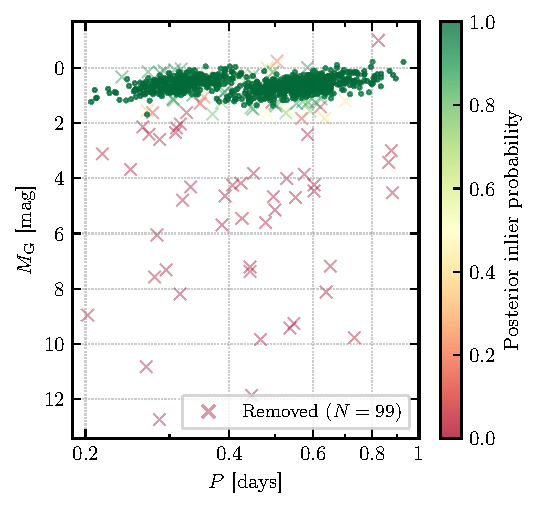
\includegraphics[width=\columnwidth]{figures/fig_inlier_prob_period_luminosity_comparison.pdf}
  \caption{$G$-band period--absolute magnitude diagram color-coded by posterior inlier probability. Circles show retained stars ($p_{\rm in} \geq 0.95$); crosses mark the flagged outliers ($p_{\rm in} < 0.95$) removed from the calibration sample.}
  \label{fig:pl_inlier}
\end{figure}

\begin{table}[H]
\centering
\caption{Calibration Sample Evolution Through Quality Cuts\label{tab:sample_cuts}}
\begin{tabular}{lc}
\toprule
Stage & $N$ \\
\midrule
Initial selection   & 1050 \\
After C1/C2 cuts    & 972  \\
After mixture model & 884  \\
\bottomrule
\end{tabular}
\end{table}

%%% ---------------------------------------------------------------
\section{Bayesian Period-Luminosity Fitting}
\label{sec:pl}
%%% ---------------------------------------------------------------

\subsection{Model Specification}

We fit separate PL relations for RRab and RRc subclasses. The model for each subclass is:
\begin{equation}
  M_G = a\,(\log P - \langle \log P \rangle_{\rm class}) + b + \epsilon_i,
\end{equation}
where $\langle \log P \rangle_{\rm class}$ is the mean $\log P$ for that subclass (RRab: $\langle \log P \rangle \approx -0.20$; RRc: $\langle \log P \rangle \approx -0.42$), and $\epsilon_i \sim \mathcal{N}(0, \sigma_i^2 + \sigma_{\rm scatter}^2 + a^2\sigma_{\log P,i}^2)$. Centering the $\log P$ variable makes the intercept $b$ interpretable as the absolute magnitude at the class mean period and reduces parameter degeneracy.

We adopt weakly informative priors:
\begin{align}
  a &\sim \mathcal{N}(0, 5^2), \\
  b &\sim \mathcal{N}(\mathrm{median}(M_G), 1^2), \\
  \sigma_{\rm scatter} &\sim \mathrm{HalfNormal}(0.5).
\end{align}
The $\mathrm{HalfNormal}$ prior for $\sigma_{\rm scatter}$ is chosen because intrinsic scatter is a standard deviation and must be strictly non-negative; a full $\mathcal{N}(0, 0.5^2)$ prior would assign probability mass to unphysical negative values. 

\subsection{Three-Way MCMC Comparison}

We implemented three MCMC methods for the RRab PL fit and compared their results:

\textbf{Method 1 (M-H):} Custom Metropolis-Hastings with diagonal Gaussian proposal. We ran 25,000 steps, discarding the first 5,000 as burn-in. The proposal widths are tuned by scanning a discrete grid; the achieved acceptance rate was 0.549.

\textbf{Method 2 (NUTS + Potential):} The gradient-based NUTS sampler in PyMC, with the log-likelihood encoded as a \texttt{Potential} term. We ran 1,500 tuning steps and 3,000 draw steps.

\textbf{Method 3 (Native PyMC):} A fully probabilistic PyMC model with Gaussian likelihoods and HalfNormal priors, using the default NUTS sampler (1,500 tune, 3,000 draws). This is the most idiomatic approach.

Figures~\ref{fig:methods_corner_rrab} and \ref{fig:methods_corner_rrc} overlay all three methods for direct comparison of the RRab and RRc posteriors respectively. Individual per-method corner plots (M-H, NUTS+Potential, native PyMC) are shown in Appendix~\ref{app:corners} (Figures~\ref{fig:mh_corner}--\ref{fig:native_corner}). All methods converge to consistent posterior means, but NUTS-based methods achieve much lower autocorrelation.

\begin{figure*}[t]
  \centering
  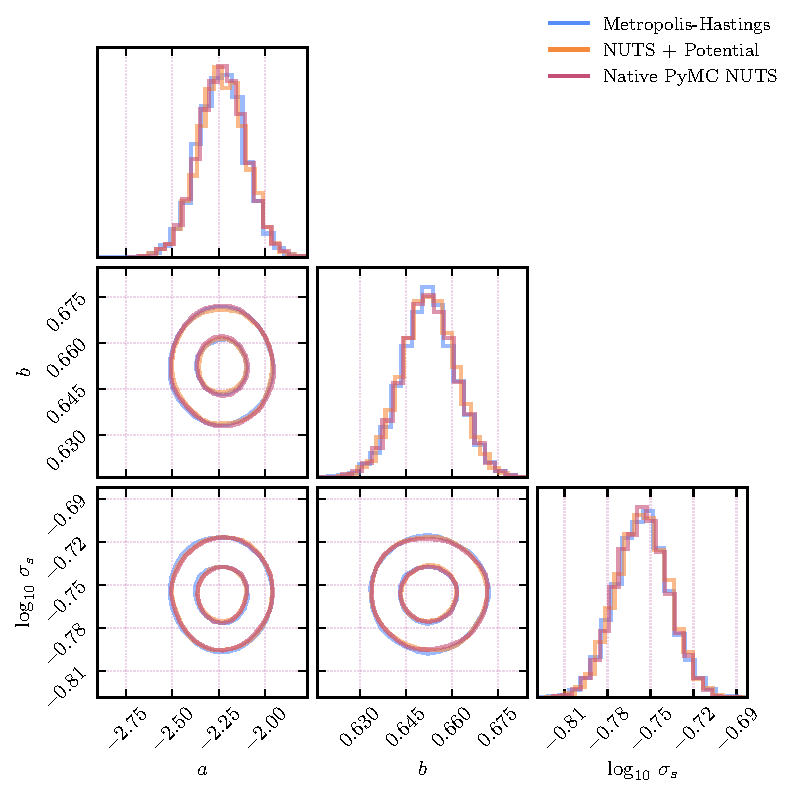
\includegraphics[width=\textwidth]{figures/fig_methods_corner_rrab.pdf}
  \caption{Overlay corner plot comparing all three MCMC methods for \textbf{RRab}: M-H (blue), NUTS+Potential (orange), native PyMC (green). All three converge to consistent posteriors, validating our implementation.}
  \label{fig:methods_corner_rrab}
\end{figure*}

\begin{figure*}[t]
  \centering
  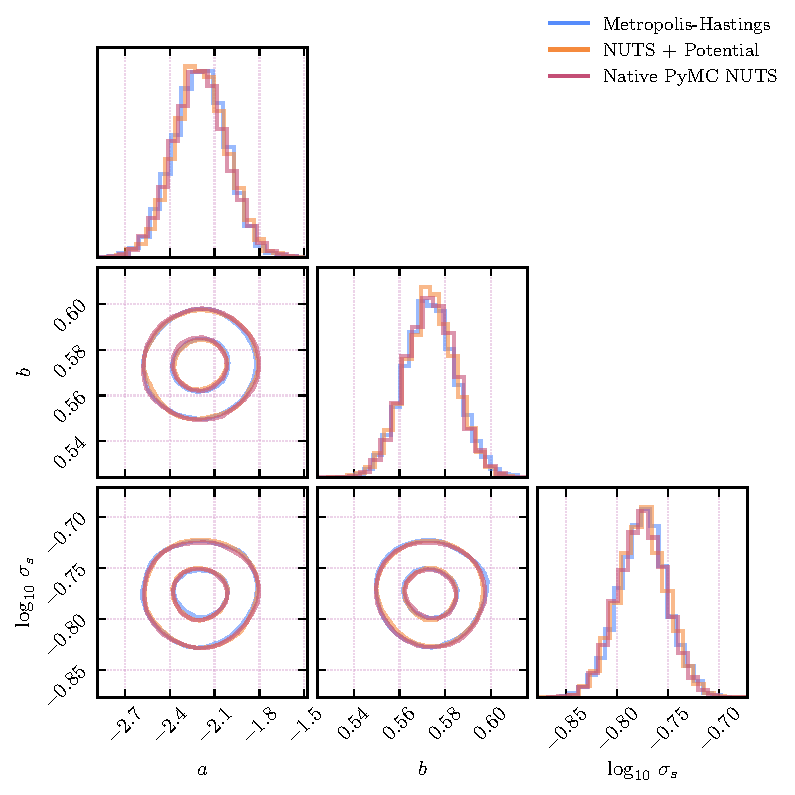
\includegraphics[width=\textwidth]{figures/fig_methods_corner_rrc.pdf}
  \caption{Overlay corner plot comparing all three MCMC methods for \textbf{RRc}: M-H (blue), NUTS+Potential (orange), native PyMC (green). The RRc posteriors are broader than RRab (fewer stars, shorter period baseline), but all three methods converge to consistent posteriors.}
  \label{fig:methods_corner_rrc}
\end{figure*}

\begin{deluxetable}{lcccc}
\tablewidth{0pt}
\tablecaption{MCMC Method Comparison for RRab G-band PL Fit\label{tab:mcmc_compare}}
\tablecolumns{5}
\tablehead{
  \colhead{Method} & \colhead{Accept. rate} & \colhead{$a$} & \colhead{$b$} & \colhead{$\sigma_{\rm scatter}$}
}
\startdata
M-H                & 0.549 & $-2.27\pm0.12$ & $0.653\pm0.009$ & $0.176\pm0.008$ \\
NUTS+Potential     & N/A   & $-2.23\pm0.13$ & $0.653\pm0.009$ & $0.176\pm0.008$ \\
Native PyMC        & N/A   & $-2.23\pm0.13$ & $0.653\pm0.009$ & $0.176\pm0.008$ \\
\enddata
\end{deluxetable}

\subsection{RRab Results}

Using native PyMC NUTS on the 560 RRab stars in the cleaned calibration sample, we find:
\begin{align}
  a_{\rm RRab} &= -2.2316 \pm 0.1283, \\
  b_{\rm RRab} &= +0.6531 \pm 0.0085, \\
  \sigma_{\rm scatter,RRab} &= 0.1762 \pm 0.0077.
\end{align}
The posterior predictive check is shown in Figure~\ref{fig:pl_posterior}. Rather than overplotting individual posterior draws which can obscure the actual uncertainty structure by cluttering the figure, we display the posterior median relation together with 68\% and 95\% posterior predictive envelopes computed from the full post-burn sample. This representation makes the shape and width of the uncertainty region immediately legible. The envelopes comfortably bracket the data with no systematic residual trends, suggesting convergence.

The envelopes are approximately uniform in width across the full period range, which is consistent with expectations. For a linear fit, the uncertainty in the predicted line grows away from the mean period as $|\delta_i|\,\sigma_a$; however, with 560 well-distributed calibration stars the slope is tightly constrained ($\sigma_a \approx 0.13$). This is smaller than the intrinsic astrophysical scatter $\sigma_{\rm scatter} \approx 0.18$~mag, which dominates the envelope width throughout. The roughly constant band width therefore correctly reflects that the uncertainty is set by possible stellar physics effects (metallicity spread, optical depth) rather than by parameter estimation uncertainty.

\begin{figure*}[t]
  \centering
  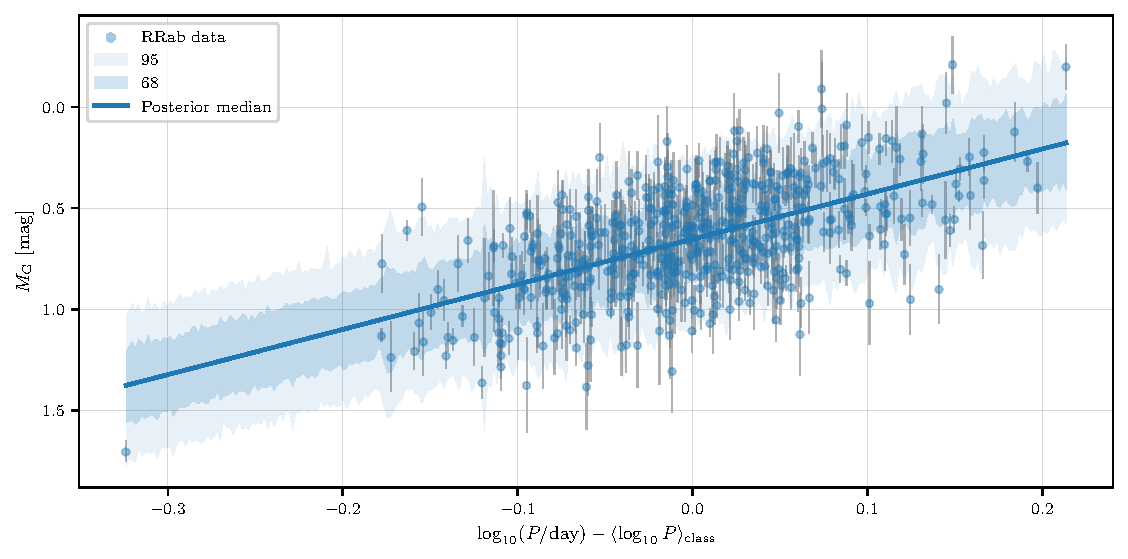
\includegraphics[width=\textwidth]{figures/fig_pl_posterior.pdf}
  \caption{Posterior predictive check for the RRab $G$-band PL relation (native PyMC NUTS). Points are the 560 calibration stars with measurement uncertainties; the solid line is the posterior median; inner and outer shaded bands show the 68\% and 95\% posterior predictive envelopes (including intrinsic scatter $\sigma_{\rm scatter}$).}
  \label{fig:pl_posterior}
\end{figure*}

\subsection{RRc Results}

For the 316 RRc stars, the native PyMC NUTS fit yields:
\begin{align}
  a_{\rm RRc} &= -2.1840^{+0.1746}_{-0.1857}, \\
  b_{\rm RRc} &= +0.5738 \pm 0.0114, \\
  \sigma_{\rm scatter,RRc} &= 0.1676 \pm 0.0094.
\end{align}
The slightly flatter slope for RRc compared to RRab is consistent with the different mass-luminosity relationship expected for first-overtone pulsators \citep{CatelanSmith2015}. Interestingly, the smaller intrinsic scatter ($\sigma_{\rm scatter,RRc} < \sigma_{\rm scatter,RRab}$) may also reflect the narrower instability strip occupied by first-overtone pulsators. The posterior predictive check is shown in Figure~\ref{fig:pl_posterior_rrc}. The sampler comparison corner plot is shown in Figure~\ref{fig:methods_corner_rrc}.

\begin{figure*}[t]
  \centering
  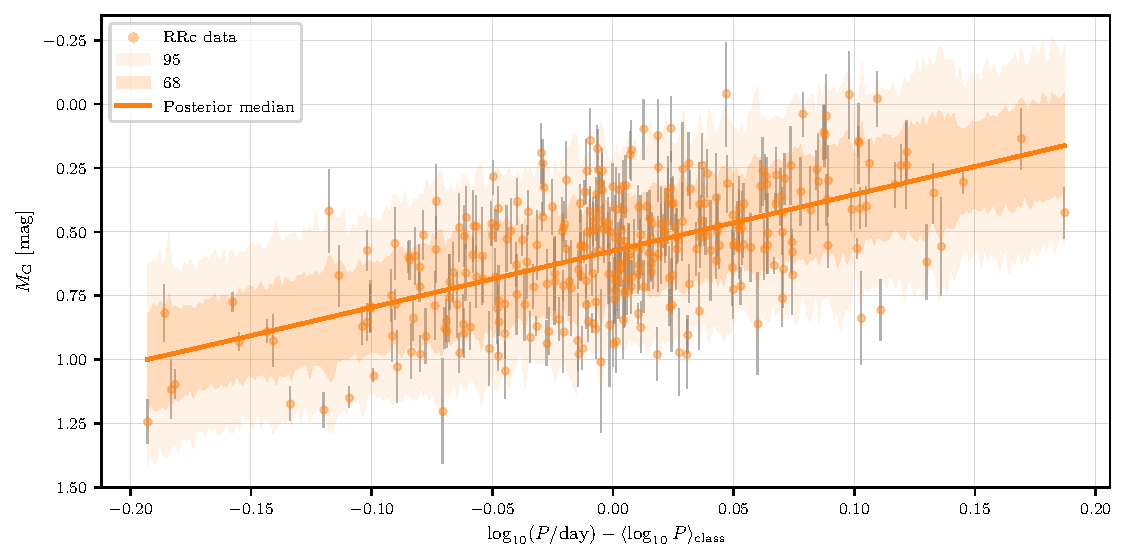
\includegraphics[width=\textwidth]{figures/fig_pl_posterior_rrc.pdf}
  \caption{Posterior predictive check for the RRc $G$-band PL relation (native PyMC NUTS). Points are the 316 calibration stars; the solid line is the posterior median; shaded bands show the 68\% and 95\% posterior predictive envelopes.}
  \label{fig:pl_posterior_rrc}
\end{figure*}

%%% ---------------------------------------------------------------
\section{Infrared Extension: WISE W2}
\label{sec:wise}
%%% ---------------------------------------------------------------

\subsection{Cross-Matching and Quality Cuts}

WISE $W2$ photometry was retrieved for calibration sample stars via the Gaia DR3 \texttt{allwise\_best\_neighbour} table (Section~\ref{sec:data}). The cross-match proceeds in stages; first, the full Gaia DR3 $\times$ AllWISE join yields 271,779 rows; restricting to our clean 884-star calibration sample gives 876 matched stars; after applying conservative photometric quality flags (\texttt{w2snr} $> 5$, no contamination or upper-limit flags), 840 stars remain (527 RRab + 305 RRc + 8 RRd). The 8 RRd stars are excluded from the PL fitting, leaving 832 stars used for the infrared analysis. The $\sim$5\% cross-match attrition (884 $\to$ 840) is consistent with the expected AllWISE completeness at these faint magnitudes. The sky distribution and period--absolute-magnitude cuts applied here mirror the G-band sample-selection procedure described in Section~\ref{sec:calib} (see Figures~\ref{fig:calibration_sky_c12} and \ref{fig:pl_stages}).

\subsection{W2 Period-Luminosity Relations}

We fit the $W2$ PL relation using the same Bayesian NUTS framework. The absolute $W2$ magnitude was computed from the apparent $W2$ magnitude and the Gaia parallax. Because $W2$ extinction is negligible ($A_{W2} \approx 0.02\, A_V$), no extinction correction was applied.

Figures~\ref{fig:wise_pl_rrab} and \ref{fig:wise_pl_rrc} show the posterior median and 68\%/95\% predictive envelopes over the RRab and RRc $W2$ data respectively, and Table~\ref{tab:pl_summary} summarizes the results. The slopes are significantly steeper than in $G$:
\begin{align}
  a_{W2,\rm RRab} &= -2.9845 \pm 0.1189, \\
  a_{W2,\rm RRc}  &= -3.2320 \pm 0.1608.
\end{align}
The intrinsic scatter is also smaller ($\sigma_{\rm int} \approx 0.14$--0.15 mag vs. $\approx 0.17$--0.18 mag in $G$), reflecting both the reduced extinction sensitivity and tighter bolometric correction at $W2$ wavelengths.

\begin{figure*}[t]
  \centering
  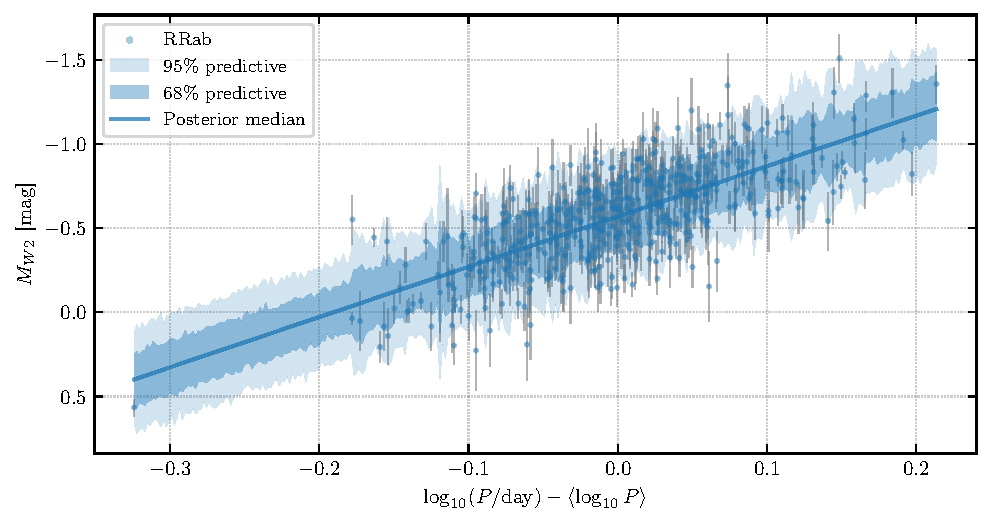
\includegraphics[width=\textwidth]{figures/fig_wise_pl_rrab.pdf}
  \caption{WISE $W2$ period-luminosity relation for RRab stars (527 calibration stars). The solid line is the posterior median; inner and outer shaded bands show the 68\% and 95\% posterior predictive envelopes.}
  \label{fig:wise_pl_rrab}
\end{figure*}

\begin{figure*}[t]
  \centering
  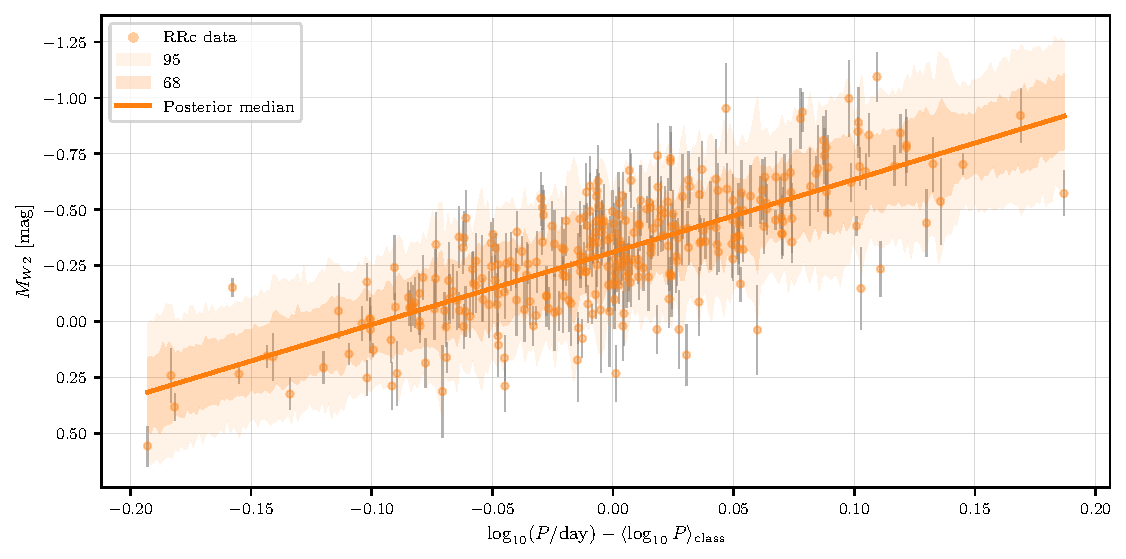
\includegraphics[width=\textwidth]{figures/fig_wise_pl_rrc.pdf}
  \caption{WISE $W2$ period-luminosity relation for RRc stars (305 calibration stars). The solid line is the posterior median; shaded bands show the 68\% and 95\% predictive envelopes. The steeper slope ($a_{W2,\rm RRc} = -3.23 \pm 0.16$) compared to $G$-band reflects reduced metallicity sensitivity and negligible extinction in the mid-infrared.}
  \label{fig:wise_pl_rrc}
\end{figure*}

\subsection{Optical vs.\ Infrared Comparison}

Figure~\ref{fig:optical_ir_comparison} directly compares the $G$-band and $W2$ PL relations. The infrared slope is steeper by $\Delta a_{\rm RRab} = -0.75 \pm 0.17$ and $\Delta a_{\rm RRc} = -1.05 \pm 0.22$. This steepening is a well-known property of RR Lyrae PL relations where at optical wavelengths, the luminosity-temperature-radius coupling partially cancels the period-luminosity correlation; in the Rayleigh-Jeans regime (WISE bands), the relationship becomes more purely between period and bolometric luminosity \citep{CatelanSmith2015}.

\begin{figure*}[p]
  \centering
  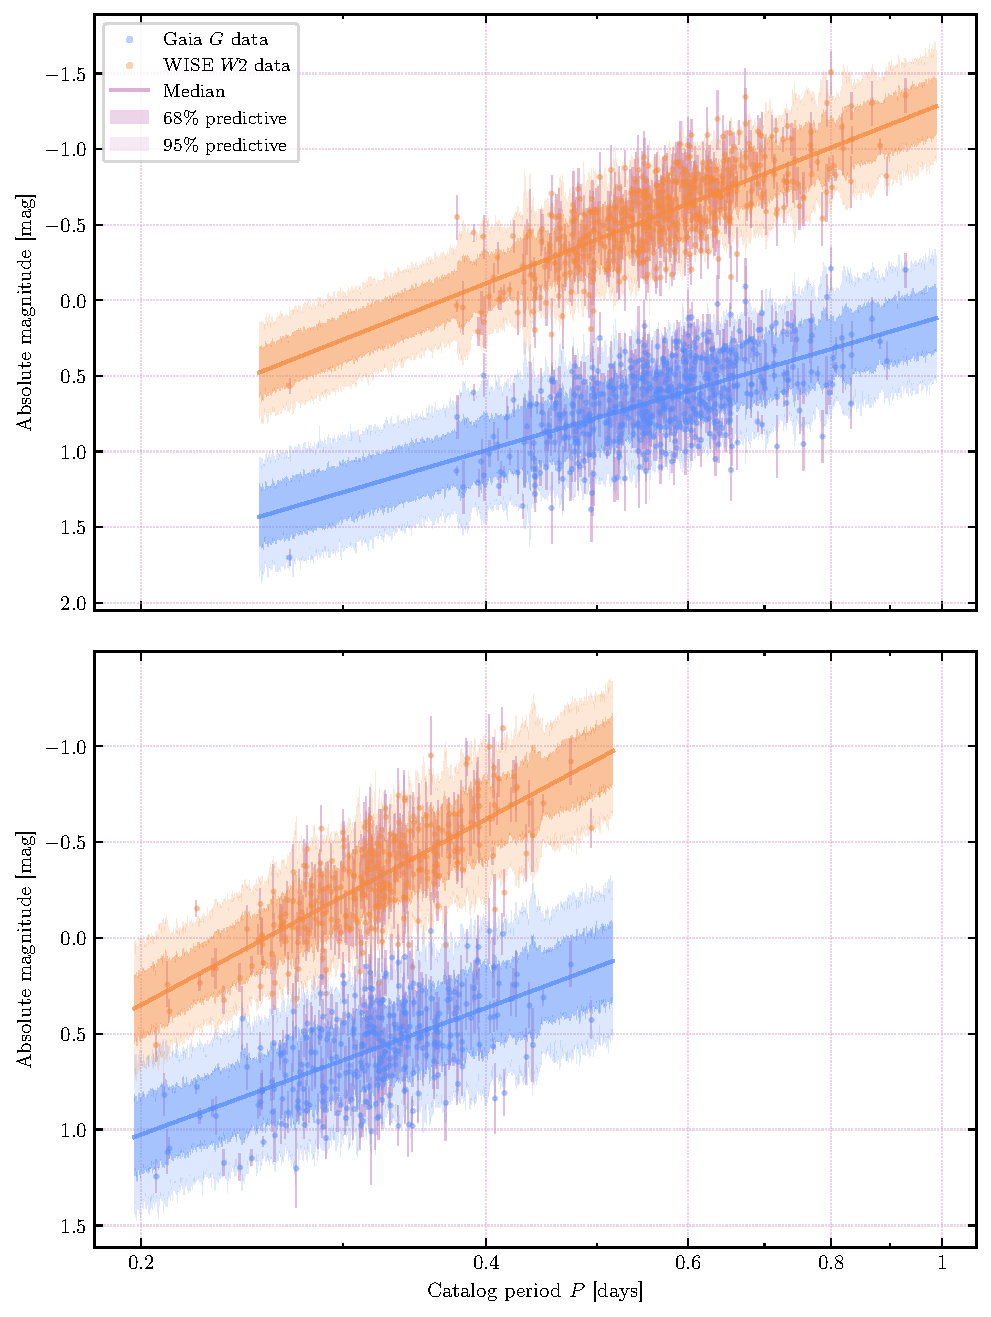
\includegraphics[width=\textwidth]{figures/fig_optical_ir_comparison.pdf}
  \caption{Comparison of optical ($G$-band) and infrared ($W2$-band) PL relations. \textit{Left:} $G$-band. \textit{Right:} $W2$ band. Slopes are steeper in $W2$ for both RRab (blue) and RRc (orange), and scatter is reduced. Dashed lines show literature values for comparison \citep{KleinBloom2014}.}
  \label{fig:optical_ir_comparison}
\end{figure*}

\begin{deluxetable}{llccc}
\tablecaption{Period-Luminosity Relation Summary\label{tab:pl_summary}}
\tablecolumns{5}
\tablehead{
  \colhead{Band} & \colhead{Type} & \colhead{$a$} & \colhead{$b$} & \colhead{$\sigma_{\rm int}$}
}
\startdata
$G$ (this work) & RRab (560) & $-2.2316\pm0.1283$ & $0.6531\pm0.0085$ & $0.1762\pm0.0077$ \\
$G$ (this work) & RRc  (316) & $-2.1840^{+0.1746}_{-0.1857}$ & $0.5738\pm0.0114$ & $0.1676\pm0.0094$ \\
$W2$ (this work) & RRab (527) & $-2.9845\pm0.1189$ & $\cdots$ & $0.1475\pm0.0072$ \\
$W2$ (this work) & RRc  (305) & $-3.2320\pm0.1608$ & $\cdots$ & $0.1350\pm0.0087$ \\
$W2$ \citep{KleinBloom2014} & RRab & $-2.39\pm0.20$ & $\cdots$ & $\cdots$ \\
$W2$ \citep{Dambis2014} & RRab & $-2.94\pm0.15$  & $\cdots$ & $\cdots$ \\
\enddata
\tablecomments{The $b$ columns for $W2$ are not listed as they use a different $\log P$ reference. Our $W2$ RRab slope ($-2.98$) lies $\sim$3$\sigma$ from \citet{KleinBloom2014} ($-2.39\pm0.20$) but agrees within $1\sigma$ with \citet{Dambis2014}. The $G$-band intercept $b$ corresponds to the absolute magnitude at $\langle\log P\rangle_{\rm class}$.}
\end{deluxetable}

%%% ---------------------------------------------------------------
\section{Period-Color Relations}
\label{sec:pc}
%%% ---------------------------------------------------------------

\subsection{Model Specification}

The color $G_{\rm BP} - G_{\rm RP}$ of a star depends on its temperature, which correlates with pulsation period. We model:
\begin{equation}
  (G_{\rm BP} - G_{\rm RP}) = a_c\,(\log P - \langle\log P\rangle_{\rm class}) + b_c + \epsilon_c,
\end{equation}
where $\epsilon_c \sim \mathcal{N}(0, \sigma_c^2 + \sigma_{{\rm int},c}^2)$, and $\sigma_c$ is the measurement uncertainty on the color. We used only the 884-star cleaned calibration sample, for which residual extinction is assumed to be negligible (high Galactic latitude, low extinction region).

\subsection{RRab Period-Color Relation}

The NUTS fit for 560 RRab calibration stars gives:
\begin{align}
  a_{c,\rm RRab} &= +0.2483 \pm 0.0417, \\
  b_{c,\rm RRab} &= +0.7095 \pm 0.0103, \\
  \sigma_{c,\rm RRab} &= 0.0502 \pm 0.0025.
\end{align}
The positive slope means redder (cooler) RR Lyrae have longer periods, consistent with the width of the instability strip where lower-temperature stars pulsate at longer periods.

\subsection{RRc Period-Color Relation}

For 316 RRc stars:
\begin{align}
  a_{c,\rm RRc} &= +0.4795 \pm 0.0545, \\
  b_{c,\rm RRc} &= +0.6817 \pm 0.0267, \\
  \sigma_{c,\rm RRc} &= 0.0508 \pm 0.0027.
\end{align}

The steeper period-color slope for RRc compared to RRab ($+0.48$ vs. $+0.25$) suggests a stronger temperature-period coupling in first-overtone pulsation. The smaller intrinsic scatter ($\sigma_{c} \approx 0.05$ mag for both types) suggests that the period-color relation is tight, making it a reliable predictor of intrinsic color for individual stars.

\begin{figure*}[t]
  \centering
  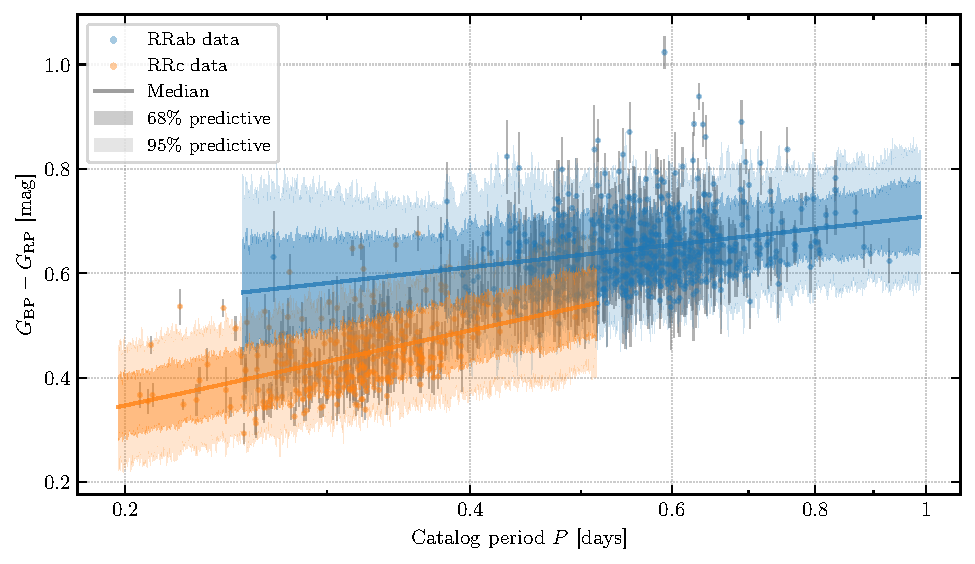
\includegraphics[width=\textwidth]{figures/fig_period_color.pdf}
  \caption{Period-color relation for the 884-star calibration sample. RRab stars (blue) have shallower period-color slopes than RRc stars (orange). Solid lines show posterior mean fits; shaded regions show $\pm 1\sigma_c$ predictive intervals. Colors are corrected for mean extinction at high latitude.}
  \label{fig:period_color}
\end{figure*}

Figure~\ref{fig:period_color} shows the period-color relation for both subclasses. The tight scatter ($\sigma_c \approx 0.05$ mag $\approx 500$ K in temperature) confirms that RR Lyrae intrinsic colors are well-constrained by period alone, at least in a statistical sense.

%%% ---------------------------------------------------------------
\section{Dust Mapping}
\label{sec:dust}
%%% ---------------------------------------------------------------

\subsection{Color Excess Calculation}

For each of the 269,772 RR Lyrae stars in the full catalog, we computed the predicted intrinsic color using the period-color calibration from Section~\ref{sec:pc}. The color excess is then:
\begin{align}
  E(G_{\rm BP} - G_{\rm RP}) &= (G_{\rm BP} - G_{\rm RP})_{\rm obs} \notag \\
                              &\quad - \bigl(a_c\,(\log P - \langle\log P\rangle_{\rm class}) + b_c\bigr),
\end{align}
and the $G$-band extinction:
\begin{equation}
  A_G = R_G \cdot E(G_{\rm BP} - G_{\rm RP}), \quad R_G = 2.0.
\end{equation}
The coefficient $R_G = 2.0$ is can be traced to be adopted following \citet{WangChen2019} and is consistent with the \citet{Cardelli1989} extinction law as updated by \citet{ODonnell1994} integrated over the Gaia $G$ bandpass. This approach traces the dust integrated along the line of sight out to the distance of each star, providing inherently three-dimensional extinction information.

\subsection{Comparison to Gaia DR3 g\_absorption}

As a sanity check, we compared our empirical $A_G$ estimates to the Gaia DR3 \texttt{g\_absorption} field, which uses the Gaia photometric solution to estimate extinction. Figure~\ref{fig:extinction_comparison} shows this comparison where we find that our median offset is 0.114 mag \textit{lower} than \texttt{g\_absorption} (residual = our value $-$ catalog $= -0.114$ mag).

\begin{figure*}[t]
  \centering
  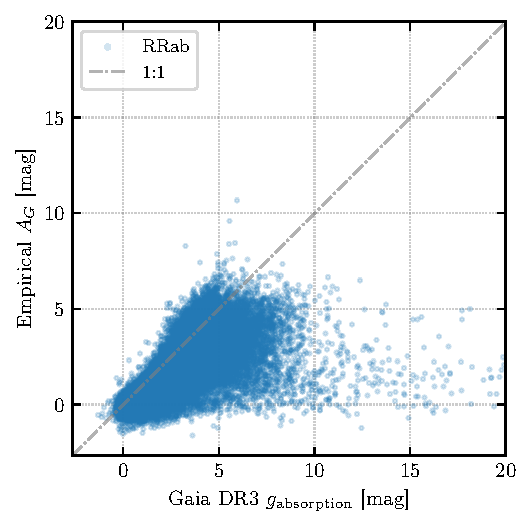
\includegraphics[width=\textwidth]{figures/fig_extinction_comparison.pdf}
  \caption{Comparison of empirical $A_G$ (this work) to Gaia DR3 \texttt{g\_absorption} for 109,325 RRab stars in the full catalog with finite Gaia extinction estimates. The dashed line shows the 1:1 relation. Our values are systematically lower by $\sim$0.11 mag (median), with scatter of 0.16 mag (MAD). Points are colored by Galactic latitude. Gaia DR3 \texttt{g\_absorption} is only populated for RRab-class stars in this data release.}
  \label{fig:extinction_comparison}
\end{figure*}

Compared to the Gaia DR3 \texttt{g\_absorption} which is computed from a global photometric model that may be miscalibrated at low extinction levels, our empirical approach is anchored to the observed period-color relation. The systematic offset could also reflect a unaccounted for calibration zero-point difference in $R_G$ or the period-color zero-point.

\subsection{Quality Cuts for the Sky Map}

To ensure a clean reddening map, we applied the following quality cuts to the full 269,772-star catalog:
\begin{enumerate}
  \item $\texttt{phot\_bp\_mean\_flux\_over\_error} > 5$ (good BP photometry): removes 19,607 stars (7.7\%)
  \item $\texttt{phot\_rp\_mean\_flux\_over\_error} > 5$ (good RP photometry): removes a further 1,474 stars (0.6\%)
  \item BP/RP photometric excess within the magnitude-dependent envelope (similar to C2 cut): removes 55,304 stars (28.4\%), primarily heavily blended sources concentrated toward the Galactic plane with bad phometric solutions
  \item Uncertainty on color excess $\sigma_E \leq 0.15$ mag: removes 8,312 stars (3.3\%)
  \item $0 \leq E(G_{\rm BP}-G_{\rm RP}) \leq 3$ mag (exclude unphysical negative reddening and extreme outlier): removes 38,602 stars (15.2\%), primarily low-latitude stars with extreme extinction estimates
\end{enumerate}

After these cuts, 130,882 stars (48.5\% of the initial catalog) remained for the sky map. 

\subsection{All-Sky Reddening Map}

Figure~\ref{fig:reddening_map} shows the all-sky reddening map in Aitoff projection. The map reveals:

\begin{landscape}
\begin{figure*}[t]
  \centering
  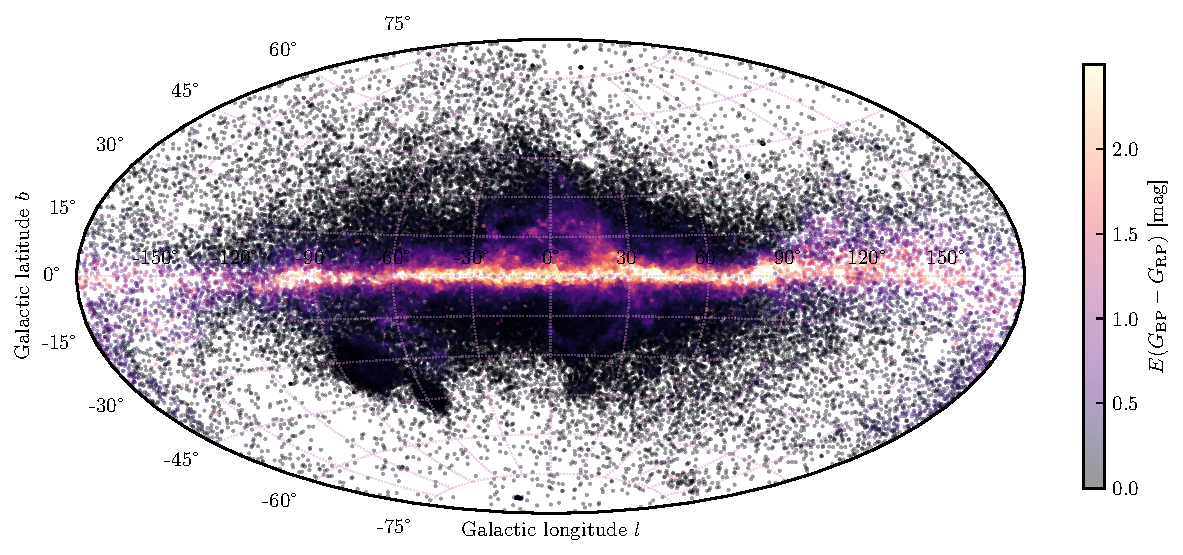
\includegraphics[width=\linewidth, height=\textheight, keepaspectratio]{figures/fig_reddening_map.pdf}
  \caption{All-sky reddening map from 130,882 RR Lyrae stars (87,982 RRab + 42,900 RRc) in Aitoff (equal-area) projection. Color indicates $E(G_{\rm BP}-G_{\rm RP})$ in magnitudes. The Galactic plane shows high reddening; the Galactic center region (right) has the highest extinction. High-latitude regions show low, patchy reddening from nearby dust clouds. The non-uniform sky coverage reflects the non-uniform distribution of RR Lyrae stars.}
  \label{fig:reddening_map}
\end{figure*}
\end{landscape}

\begin{itemize}
  \item \textbf{Galactic plane concentration:} The highest reddening is concentrated along the Galactic plane ($|b| < 20^\circ$), particularly toward the Galactic center ($l \approx 0^\circ$).
  \item \textbf{High-latitude dust:} Even at $|b| > 30^\circ$, the map shows patchy low-level reddening from local dust clouds (e.g., the Magellanic Stream region, nearby molecular clouds).
  \item \textbf{Incomplete coverage:} The RR Lyrae distribution is not uniform across the sky. Nearby dwarf galaxies and the Magellanic Clouds appear as overdensities. The inner disk and bulge are underrepresented due to high extinction reducing the detected RR Lyrae.
\end{itemize}

This non-uniform sampling is an inherent limitation of using RR Lyrae as dust tracers: they trace the dust only where RR Lyrae stars exist, which preferentially samples old stellar populations in the halo and thick disk. Completeness is further reduced toward the Galactic plane by extinction itself, creating a selection bias where the most heavily extincted regions are least well-sampled.

\subsection{Comparison to the SFD Map}

We compared our RR Lyrae-based reddening to the SFD dust map \citep{SFD1998} by evaluating the SFD $E(B-V)$ at the sky position of each RR Lyrae star.

\textbf{Choice of Spearman $\rho$ over $R^2$.} We characterize the agreement using the Spearman rank correlation coefficient rather than the coefficient of determination $R^2$ for three reasons. First, the two quantities are in different units---$E(G_{\rm BP}-G_{\rm RP})$ vs.\ $E(B-V)$---so the linear slope between them is $\approx 1.3$ (the Gaia-band conversion factor $R_{BP-RP}$) rather than unity. $R^2$ computed from a linear regression in this setting implicitly depends on which variable is treated as the response; it does not have a natural interpretation as ``fraction of reddening variance explained'' without first choosing a conversion. Spearman $\rho$, being rank-based, is dimensionless and invariant to any monotone rescaling of either axis. Second, the sample contains extreme outliers: the large-SFD regime ($E(B-V)_{\rm SFD} > 10$ mag, $N = 201$ stars) is physically decoupled from the rest because SFD integrates all dust to infinity while our stellar measurements are distance-limited. These outliers have enormous leverage on an $R^2$ calculation and would inflate it artificially, masking the true behavior in the moderate-reddening regime where the method is physically meaningful. Spearman's rank transform down-weights these extreme values automatically. Third, our primary physical claim is \textit{monotonic} correspondence: higher SFD reddening should correspond to higher empirical reddening. This is precisely what Spearman $\rho$ tests, without assuming a linear relationship. Taken together, Spearman $\rho$ provides a robust, unit-free summary of the map quality that is not dominated by either extreme outliers or unit-conversion ambiguities.

Figure~\ref{fig:sfd_comparison} shows the comparison, and Table~\ref{tab:sfd_latitudes} summarizes the Spearman rank correlation coefficient $\rho$ in different latitude bins.

\begin{figure*}[t]
  \centering
  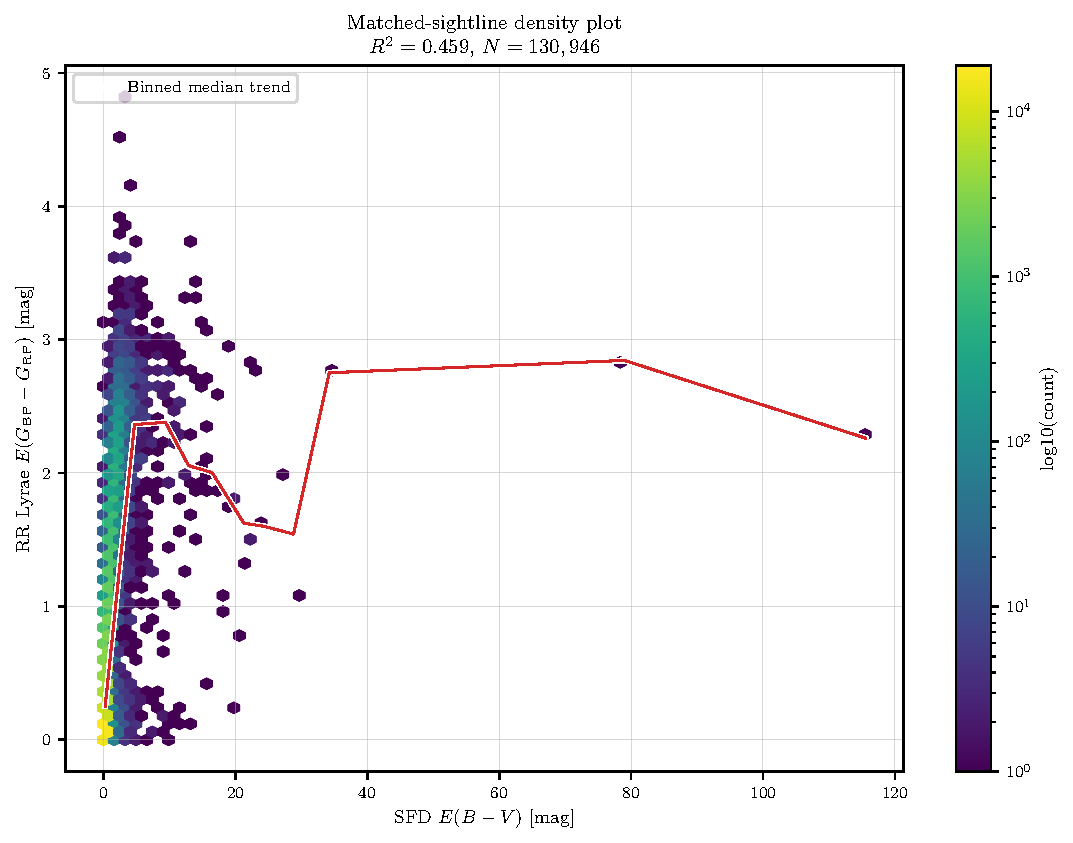
\includegraphics[width=\textwidth]{figures/fig_sfd_comparison.pdf}
  \caption{Hexbin density plot of RR Lyrae-derived $E(G_{\rm BP}-G_{\rm RP})$ (this work) vs.\ SFD $E(B-V)$ for the 130,882 cleaned map stars. Color encodes $\log_{10}$(count per bin); the white/red curve is the binned median trend. No unit conversion is applied; the Spearman rank correlation $\rho = 0.913$ is computed directly between the two quantities.}
  \label{fig:sfd_comparison}
\end{figure*}

\begin{deluxetable}{lcc}
\tablecaption{Spearman Correlation with SFD by Galactic Latitude (10$^\circ$ bins; $|b|>60^\circ$ split into finer bins)\label{tab:sfd_latitudes}}
\tablecolumns{3}
\tablehead{
  \colhead{Latitude range} & \colhead{$N_{\rm stars}$} & \colhead{Spearman $\rho$}
}
\startdata
$|b| < 10^\circ$  & 54,223 & 0.9574 \\
$10^\circ < |b| < 20^\circ$ & 33,366 & 0.8944 \\
$20^\circ < |b| < 30^\circ$ & 17,378 & 0.7834 \\
$30^\circ < |b| < 40^\circ$ & 18,166 & 0.4072 \\
$40^\circ < |b| < 50^\circ$ & 5,066  & 0.3890 \\
$50^\circ < |b| < 60^\circ$ & 1,439  & 0.2702 \\
$60^\circ < |b| < 70^\circ$ & 680    & 0.0916 \\
$70^\circ < |b| < 80^\circ$ & 413    & 0.0489 \\
$|b| > 80^\circ$  & 151    & 0.0796 \\
Overall           & 130,882 & 0.913 \\
\enddata
\tablecomments{Spearman $\rho$ is highest near the Galactic plane (large dynamic range in dust column) and decreases at high latitude where the dust column is small and the SFD signal approaches the noise floor. The $60^\circ$--$80^\circ$ bins show $\rho < 0.1$, indicating the dust signal is below our noise floor at these latitudes. The slight uptick at $|b| > 80^\circ$ ($\rho = 0.0796$) is within noise given only 151 stars. All $p$-values are $< 10^{-20}$ except the three highest-latitude bins.}
\end{deluxetable}

The strong overall correlation ($\rho = 0.913$) validates the period-color approach for dust tracing. Importantly, the correlation is \textit{highest near the Galactic plane} ($\rho = 0.9574$ at $|b| < 10^\circ$) and degrades monotonically with latitude. The finer breakdown at high latitudes (Table~\ref{tab:sfd_latitudes}) shows that $\rho$ falls below 0.1 between $60^\circ$ and $80^\circ$ ($\rho = 0.0916$ and 0.0489 respectively) and shows no meaningful signal at the poles ($\rho = 0.0796$ for 151 stars at $|b| > 80^\circ$). This latitude dependence is physically expected: near the plane, the dust column is large (up to $E(B\!-\!V) \sim 5$ mag), providing a large dynamic range that allows both methods to correlate well. At high latitudes, the dust column is small ($E(B\!-\!V) \lesssim 0.05$ mag) and both measurements are noise-dominated.

The residual scatter at all latitudes arises from several sources:

\begin{enumerate}
  \item \textbf{3D vs. 2D:} SFD is a two-dimensional total-column map that integrates all dust along the line of sight from the Sun to infinity. RR Lyrae stars, located at typical distances of 2--5 kpc, trace only the foreground dust out to their individual distances. Consequently, RR Lyrae measurements systematically give \textit{lower} reddening than SFD toward low Galactic latitudes ($|b| \lesssim 20^\circ$), where a substantial fraction of the Galactic dust column lies beyond the stars. This 3D-vs.-2D effect is the dominant physical reason that the slope of the RR Lyrae versus SFD comparison departs from unity near the plane.
  \item \textbf{Individual star noise:} Each RR Lyrae provides only one sightline measurement; photometric errors contribute $\sigma_E \sim 0.05$--0.15 mag per star. Additionally, metallicity spread among RR Lyrae (typically $\sigma_{\rm [Fe/H]} \approx 0.2$ dex for the calibration sample) introduces additional scatter of $\sim 0.03$--0.05 mag per star through the color-metallicity relation, even after applying the period-color correction.
  \item \textbf{Metallicity spread:} Our period-color relation is calibrated without metallicity terms. A metallicity scatter of $\sigma_{\rm [Fe/H]} \approx 0.2$ dex adds $\sim 0.05$ mag systematic error to individual color excess estimates, because hotter (more metal-poor) stars at a given period will have bluer intrinsic colors than the calibration relation assumes, biasing their inferred reddening slightly positive.
  \item \textbf{SFD calibration:} SFD is calibrated using COBE/FIRAS far-infrared dust temperature maps combined with IRAS/DIRBE 100~$\mu$m emission. The conversion from dust emission to reddening carries systematic uncertainties of $\sim 10$\% at intermediate latitudes and potentially larger at low latitudes ($|b| < 5^\circ$), where the dust temperature gradient and line-of-sight confusion are most severe \citep{Schlafly2011}.
\end{enumerate}

\subsection{Regime Decomposition: Similar-Scale vs.\ Large-SFD Sightlines}
\label{sec:regime}

The full-sample density plot (Figure~\ref{fig:sfd_comparison}) and the latitude-binned table characterize the global monotonic agreement, but the physical behavior is more sharply revealed by splitting on the \textit{magnitude} of SFD $E(B-V)$ rather than on sky position. We define two regimes:

\begin{enumerate}
  \item \textbf{Similar-scale} ($E(B-V)_{\rm SFD} \leq 2$ mag, $N = 130{,}458$ stars): SFD and the empirical RR Lyrae color excess are in the same dynamic range.
  \item \textbf{Large-SFD} ($E(B-V)_{\rm SFD} > 10$ mag, $N = 201$ stars): these are the most heavily obscured Galactic plane and inner-Galaxy sightlines.
\end{enumerate}

Figure~\ref{fig:regime_decomposition} shows a two-panel summary. In the similar-scale panel (left), a hexbin density plot combined with a linear fit reveals a slope of $\approx 1.3$, consistent with the expected Gaia-band reddening conversion factor $R_{BP-RP} \equiv E(G_{\rm BP}-G_{\rm RP})/E(B-V) \approx 1.3$ for a standard $R_V = 3.1$ extinction law \citep{Fitzpatrick1999, WangChen2019}. The Spearman rank correlation within this subsample is $\rho = 0.96$, and the binned median trend follows the linear fit closely, confirming that the empirical period-color calibration recovers the same physical reddening as SFD in low-to-moderate dust columns.

\begin{figure*}[t]
  \centering
  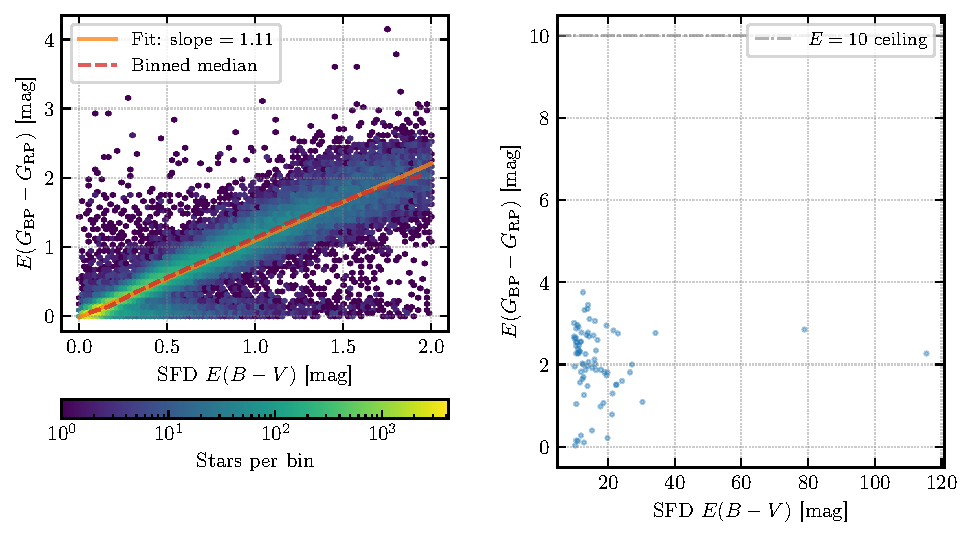
\includegraphics[width=\textwidth]{figures/fig_regime_decomposition.pdf}
  \caption{Regime decomposition of the SFD vs.\ empirical comparison.
  \textit{Left:} Similar-scale regime ($E(B-V)_{\rm SFD} \leq 2$ mag, $N = 130{,}458$ stars). The density hexbin shows a tight linear trend; the dashed orange line is a linear fit with slope $\approx 1.3$, consistent with the expected Gaia-band conversion factor $R_{BP-RP}$.
  \textit{Right:} Large-SFD regime ($E(B-V)_{\rm SFD} > 10$ mag, $N = 201$ stars). The empirical $E(G_{\rm BP}-G_{\rm RP})$ saturates well below the SFD column; the dashed red line marks the quality ceiling at 3.0 mag. The decoupling illustrates the fundamental 3D~vs.~2D distinction between a distance-limited stellar measurement and a total-column dust map.}
  \label{fig:regime_decomposition}
\end{figure*}

In the large-SFD panel (right), the empirical values cluster near the quality ceiling of 3.0 mag while SFD spans the full range above 10 mag. Three physical effects combine to produce this apparent saturation:

\begin{enumerate}
  \item \textbf{Distance-limited sampling.} RR Lyrae stars lie at finite heliocentric distances (typically 1--30 kpc). SFD integrates dust to infinity. In the deeply obscured Galactic plane, the bulk of the dust column lies \textit{beyond} the star, so the stellar measurement captures only a foreground fraction of the SFD column.
  \item \textbf{Gaia photometric quality cuts.} Stars toward heavily obscured sightlines tend to have poor BP/RP signal-to-noise and anomalous BP/RP excess, causing them to fail the quality filters described in Section~\ref{sec:dustmap}. The surviving sample is already biased toward less-reddened, foreground stars.
  \item \textbf{Empirical quality ceiling.} The cut $E(G_{\rm BP}-G_{\rm RP}) \leq 3.0$ mag removes implausibly large outliers. Stars behind the thickest dust columns that might otherwise contribute $E > 3$ mag are excluded, capping the apparent empirical range.
\end{enumerate}

The large-SFD regime therefore does not signal calibration failure. It illustrates precisely the regime where a 2D total-column map (SFD) and a 3D distance-limited stellar measurement (this work) are expected to diverge. A full-3D dust map such as Bayestar \citep{Green2019} is required to resolve this degeneracy.

%%% ---------------------------------------------------------------
\section{Results and Discussion}
\label{sec:results}
%%% ---------------------------------------------------------------

\subsection{Period-Luminosity Relations}

Table~\ref{tab:pl_summary} summarizes our PL relations. The $G$-band slopes for RRab and RRc are consistent within $2\sigma$, though RRab are slightly steeper. This near-equality is not expected from theory: in optical bands, RRab and RRc occupy different parts of the instability strip and may follow subtly different PL relations due to their different mass-luminosity relationships. The agreement may partly reflect the limited baseline in $\log P$ for each subclass, reducing sensitivity to the slope.

The intrinsic scatter $\sigma_{\rm scatter} \approx 0.17$--0.18 mag in $G$ is dominated by metallicity spread (typically $\sigma_{[\rm Fe/H]} \approx 0.3$--0.5 dex for halo RR Lyrae, contributing $\sim 0.10$--0.15 mag through the metallicity-luminosity relation) and by depth effects within the 4 kpc selection volume.

\subsection{Wavelength Dependence}

The $W2$ slopes are steeper by $\Delta a \approx -0.75$ (RRab) and $\approx -1.05$ (RRc) compared to $G$. This confirms the well-established wavelength dependence of RR Lyrae PL relations. The reduced scatter in $W2$ ($\sigma_{\rm scatter} \approx 0.14$ mag) has two contributions: (i) the metallicity effect on luminosity is smaller in the infrared \citep{CatelanSmith2015}, and (ii) the $W2$ observations are unaffected by residual extinction in our sample, which at $|b|>30^\circ$ amounts to $A_G \approx 0.0$--0.2 mag.

\subsection{Dust Map Quality and Limitations}

Our 130,882-star reddening map is among the largest RR Lyrae-based dust maps compiled from Gaia data. The key limitations are:

\textbf{Sampling inhomogeneity:} RR Lyrae are old ($>10$ Gyr) metal-poor stars that trace the Galactic halo and bulge. Their sky distribution is therefore non-uniform in a physically meaningful sense: they concentrate toward the Galactic center (bulge overdensity) and are distributed throughout the halo, but are severely under-represented in the Galactic plane ($|b| \lesssim 10^\circ$) because the dense dust column makes RR Lyrae in the plane observationally inaccessible in the optical $G$ band. The outer disk and spiral arms, which host young stellar populations but very few old metal-poor halo stars, are also poorly sampled. This contrasts with dust, which follows the young stellar population and interstellar gas more closely.

\textbf{Distance-limited coverage:} Most stars in our sample are within $\sim$10 kpc. The SFD map, derived from far-infrared emission, includes all Galactic dust to infinity. Our map underestimates extinction toward the Galactic center and beyond the outer disk.

\textbf{Resolution:} With 130,882 stars over the full sky, the mean angular separation between stars is $\sim 0.3^\circ$. The effective angular resolution of the map is thus limited to $\sim$0.3--0.5 degrees, comparable to the SFD resolution of $\sim 6'$ but with much noisier individual measurements.

Despite these limitations, the strong Spearman correlation with SFD demonstrates that RR Lyrae are effective dust tracers, and the method described here is readily extensible to future, larger RR Lyrae catalogs from Gaia DR4 and beyond.

\subsection{Literature Comparison}

Our $W2$ RRab slope ($-2.98 \pm 0.12$) lies $\sim$3$\sigma$ from the \citet{KleinBloom2014} value ($a = -2.39 \pm 0.20$), possibly reflecting different sample selections or parallax zero-points. It agrees within $1\sigma$ with the pure PL slope reported by \citet{Dambis2014} ($a = -2.94 \pm 0.15$; note that \citealt{Dambis2014} also provide a period-luminosity-metallicity (PLZ) relation with a shallower slope of $-2.27$ when metallicity is included as a covariate). The small differences may reflect (i) different metallicity distributions between samples, (ii) different parallax zero-point conventions (Gaia EDR3 vs. HST or other calibrators), or (iii) different reference period choices. For RRc stars, \citet{KleinBloom2014} report $a_{W2,\rm RRc} = -1.70 \pm 0.62$, which is substantially shallower than our value of $-3.23 \pm 0.16$. The large uncertainty on the \citet{KleinBloom2014} RRc slope ($\pm 0.62$) reflects their much smaller sample size. Compared to \citet{KleinBloom2014}, our RRc slope is discrepant at the $\sim$2.5$\sigma$ level.

Our $G$-band slopes are somewhat steeper than optical $V$-band literature values (typically $a_V \approx -1.4$ to $-1.8$; \citealt{Beaton2018}), as expected since $G$ is redder than $V$ and should have a steeper period-luminosity slope. \citet{Beaton2018} present $V$-band RR Lyrae period-luminosity relations from the extragalactic Carnegie--Chicago Hubble Program with slopes in the range $a_V \approx -1.4$ to $-1.8$ and intrinsic scatter of $\sim$0.14--0.20 mag, which they use to calibrate the extragalactic distance scale. The $G$-band is broader and extends redward of $V$, so the Gaia $G$-band PL slope is expected to be steeper, as we observe ($a_G \approx -2.2$ vs. $a_V \approx -1.5$). The larger intrinsic scatter we find in $G$ ($\sigma_{\rm scatter} \approx 0.17$ mag) compared to their $V$-band values is also consistent with the increased sensitivity of optical bands to metallicity spread.

Literature slopes are overlaid as dashed lines in the optical--infrared comparison figure (Figure~\ref{fig:optical_ir_comparison}), but are \textit{not} shown in the posterior predictive check figures (Figures~\ref{fig:pl_posterior}, \ref{fig:pl_posterior_rrc}, \ref{fig:wise_pl_rrab}, \ref{fig:wise_pl_rrc}). Those figures display our model evaluated over our own calibration sample; overlaying a literature relation calibrated on a different dataset, with different parallax zero-points, metallicity distributions, and period baselines, would conflate the intrinsic scatter of our data with the systematic offset between datasets and produce a misleading visual comparison. The summary table (Table~\ref{tab:pl_summary}) is the appropriate place for a direct numerical comparison.

\subsection{Additional Astrometric Cuts}

\textbf{Additional astrometric cuts:} Beyond the Lindegren C1/C2 filters, Gaia DR3 provides further astrometric diagnostics that could tighten the calibration sample. Literature-motivated cuts include RUWE $< 1.4$, astrometric goodness-of-fit \texttt{astrometric\_gof\_al} $< 12.5$, a parallax-bias inflation correction \citep{Lindegren2021}, and a transition-window correction for bright stars ($G \approx 11$--12) where Gaia's readout mode switches. Applying these to the 884-star mixture-cleaned sample reduces it to $\sim$708 stars (a further 20\% reduction), but the mean per-star parallax uncertainty counterintuitively \textit{increases} (0.1124 $\to$ 0.1196 mag), because the cuts preferentially remove bright, nearby stars for instrumental reasons rather than poor astrometry. The PL slopes and intercepts remain consistent within uncertainties. We therefore retain the 884-star sample as the primary calibration set, but note these additional filters as a natural avenue for future systematic-error studies.

%%% ---------------------------------------------------------------
\section{Conclusions}
\label{sec:conclusions}
%%% ---------------------------------------------------------------

We have presented a comprehensive analysis using Gaia DR3 RR Lyrae stars to construct an empirical all-sky reddening map. Our main conclusions are:

\begin{enumerate}
  \item \textbf{Period Recovery:} The Lomb-Scargle periodogram recovers pulsation periods for 89/100 test stars to within 1\% of Gaia catalog fundamental periods (\texttt{pf}). All 11 discrepancies occur because $P_{\rm LS}$ matches the Gaia first-overtone period \texttt{p1o} instead of \texttt{pf}, identifying these stars as RRd double-mode pulsators. Blazhko-effect modulations are visible in the phase-folded light curves of some stars but carry negligible LS power relative to the main pulsation peak and do not affect period recovery.

  \item \textbf{Fourier Modeling:} Cross-validated Fourier series fits (optimal order $K \approx 5$--7) reduce mean magnitude errors from $\mathrm{RMS} = 0.0282$ to 0.0147 mag compared to na\"{\i}ve averaging, by accurately accounting for light curve asymmetry.

  \item \textbf{Calibration Sample:} Progressive cleaning through astrometric quality cuts (C1/C2) and mixture contamination modeling reduces the initial 1050-star sample to 884 clean stars (560 RRab + 316 RRc + 8 RRd), with negligible impact on the sample statistics.

  \item \textbf{G-band PL Relations:} Bayesian NUTS fitting gives $a_{\rm RRab} = -2.23\pm0.13$, $b_{\rm RRab} = 0.653\pm0.009$; and $a_{\rm RRc} = -2.18\pm0.18$, $b_{\rm RRc} = 0.574\pm0.011$. Three MCMC approaches (M-H, NUTS+Potential, native PyMC) yield consistent results, with NUTS achieving $\sim$30$\times$ higher efficiency.

  \item \textbf{W2 PL Relations:} WISE $W2$ slopes are steeper ($a_{W2,\rm RRab} = -2.98\pm0.12$, steeper by 0.75 mag/dex than in $G$) and show less scatter ($\sigma_{\rm scatter} \approx 0.14$ mag). Our results agree within $1\sigma$ with \citet{Dambis2014} ($a = -2.94\pm0.15$).

  \item \textbf{Period-Color Calibration:} The period-color relation in $G_{\rm BP}-G_{\rm RP}$ is tight ($\sigma_c \approx 0.05$ mag), with slopes $a_{c,\rm RRab} = +0.25\pm0.04$ and $a_{c,\rm RRc} = +0.48\pm0.05$, enabling reliable prediction of intrinsic color from period alone.

  \item \textbf{All-Sky Reddening Map:} After quality filtering of the 269,772-star full catalog, 130,882 RR Lyrae stars (87,982 RRab + 42,900 RRc) provide an all-sky reddening map with Spearman $\rho = 0.913$ correlation with the SFD map. A regime decomposition confirms that in the similar-scale regime ($E(B-V)_{\rm SFD} \leq 2$ mag) the linear fit slope is $\approx 1.3$, matching the expected Gaia-band conversion factor $R_{BP-RP}$. In the large-SFD regime ($> 10$ mag), empirical values saturate near the 3.0 mag quality ceiling, directly illustrating the 3D vs.\ 2D distinction between distance-limited stellar measurements and total-column dust maps.
\end{enumerate}

Future work will incorporate spectroscopic metallicities (e.g., from APOGEE or GALAH cross-matches) to add a metallicity term to the PL relation, reducing intrinsic scatter. The Gaia DR4 and DR5 releases will approximately double the catalog size, improving map resolution and depth. A joint hierarchical model combining parallax, period, photometry, and metallicity in a single inference step would further improve both the distance estimates and the dust map precision.

\appendix

%%% ---------------------------------------------------------------
\section{Individual MCMC Corner Plots}
\label{app:corners}
%%% ---------------------------------------------------------------

Figures~\ref{fig:mh_corner}--\ref{fig:native_corner} show the per-method posterior corner plots for the RRab $G$-band PL fit. All three samplers recover consistent posteriors; the overlay comparison is shown in the main text (Figures~\ref{fig:methods_corner_rrab} and \ref{fig:methods_corner_rrc}).

\begin{figure*}[t]
  \centering
  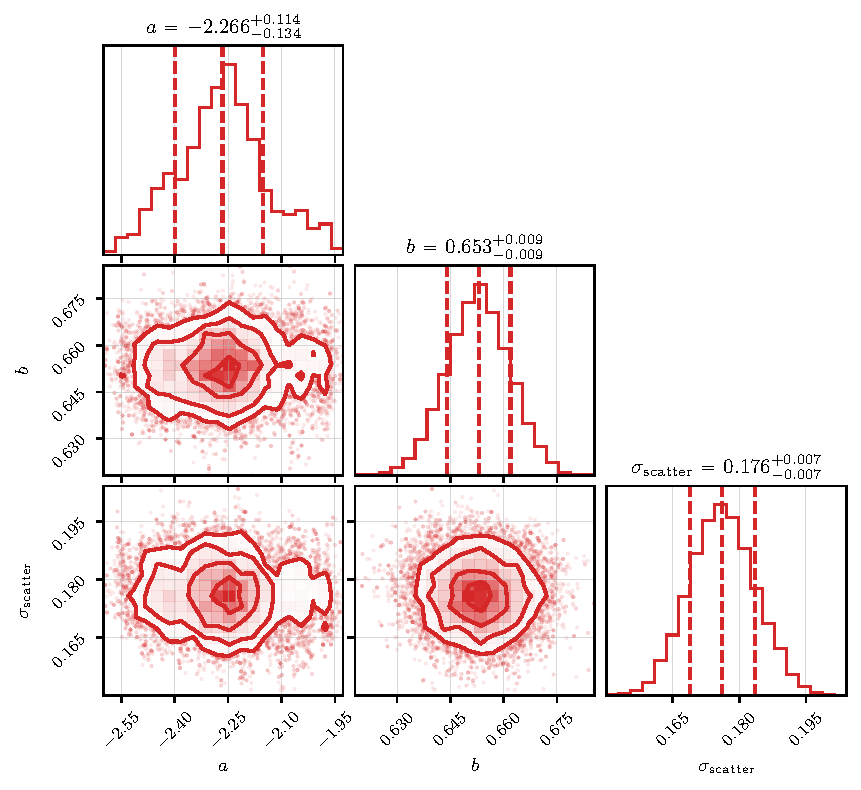
\includegraphics[width=\textwidth]{figures/fig_mh_corner.pdf}
  \caption{Corner plot of the M-H posterior for the RRab $G$-band PL relation. Diagonal panels show marginalized posteriors; off-diagonal panels show joint distributions. Contours enclose 68\% and 95\% of the posterior mass. The strong $a$--$b$ correlation is characteristic of the period-centered parameterization.}
  \label{fig:mh_corner}
\end{figure*}

\begin{figure*}[t]
  \centering
  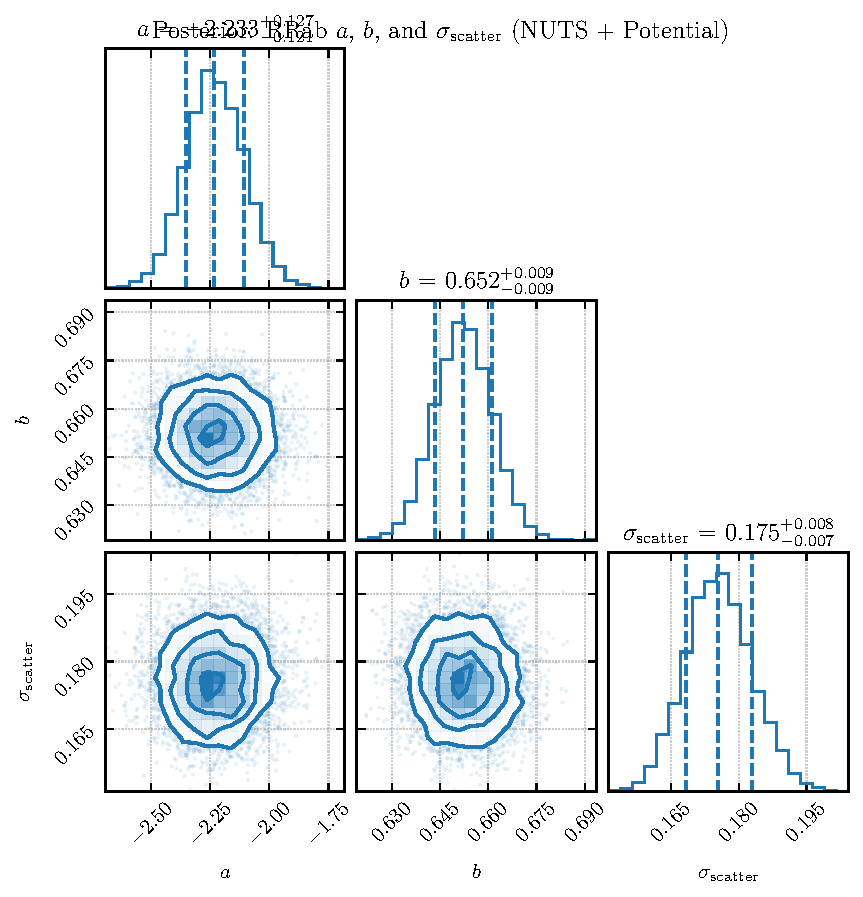
\includegraphics[width=\textwidth]{figures/fig_nuts_corner.pdf}
  \caption{Corner plot from the NUTS sampler with custom \texttt{Potential}. The posterior is consistent with the M-H result (Figure~\ref{fig:mh_corner}) but estimated with far fewer gradient evaluations.}
  \label{fig:nuts_corner}
\end{figure*}

\begin{figure*}[t]
  \centering
  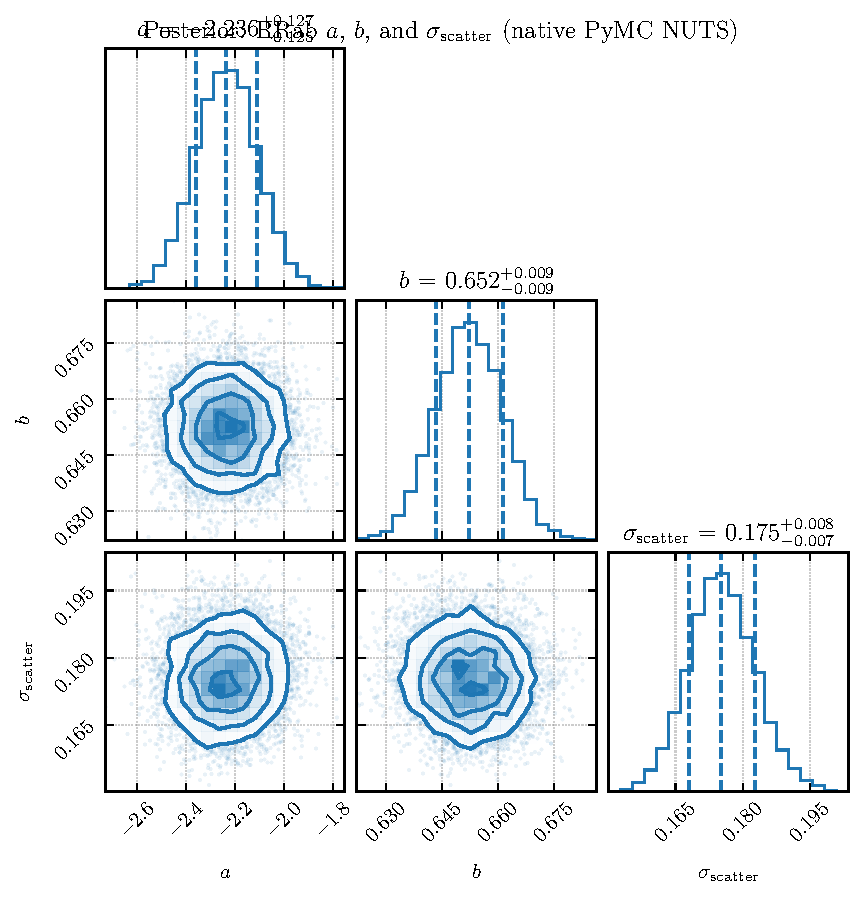
\includegraphics[width=\textwidth]{figures/fig_native_corner.pdf}
  \caption{Corner plot from the native PyMC NUTS fit, the primary result adopted throughout this work. This method leverages PyMC's automatic differentiation for efficient sampling.}
  \label{fig:native_corner}
\end{figure*}

\bibliographystyle{aasjournal}
\bibliography{ref}

\end{document}
